
\documentclass[conference,letterpaper,10pt,top=0.7in]{IEEEtran}
%\documentclass[journal,draftcls,onecolumn,12pt,twoside]{IEEEtran}
\newcommand{\folder}{/home/bohulu/Documents/texmf}
%\newcommand{\folder}{/home/hanchenggao/Documents/texmf}
\input{\folder/hfiles/epaper}
\usepackage {graphics}
\usepackage{caption}
\usepackage{tabularx}
\begin{document}
\title{
A Method to Determine the Patterns of Low-Weight Codewords for Recursive Systematic Convolutional Codes}
\author{%
  \IEEEauthorblockN{Kwame~Ackah~Bohulu~and~Chenggao~Han\\}
  \IEEEauthorblockA{Graduate School of Informatics and Engineering,\\
   The University of Electro-Communications,\\
    1-5-1 Chofugaoka, Chofu-shi, Tokyo, 182--8585, Japan\\
                    Email: \{bohulu, han.ic\}@uec.ac.jp}
}


\maketitle
\begin{abstract}
For the turbo code (TC) consisting of  recursive systematic convolutional (RSC) codes, the complete knowledge of the low-weight codewords of the RSC code is very important for interleaver design in order to achieve good TC performance. In this paper, we present a method to determine the patterns of low-weight codewords for  RSC codes. For a given RSC code, we first identify the codewords with weight-$2$ and weight-$3$ parity-check components (PCs) based on the characteristic of the feed-forward polynomial. Similarly, we identify the codewords with low-weight systematic components (SCs) based on the feedback polynomial, and then establish the low-weight codewords from the identified codewords. To validate our proposed method, we obtain a union bound using the established low-weight codewords and compare it with that obtained via the transfer function method and the bit error rate (BER) curve drawn from simulation results.
\end{abstract}
\section{Introduction}

The {\it turbo code} (TC) \cite{ref1}, introduced by Claude Berrou in 1993 is one of the forward-error correcting codes that comes very close to satisfying the Shannon limit for AWGN channels.  Due to its excellent performance, TCs have been used in many applications and  adopted as the channel code for the LTE standard, IEEE 802.16 WiMAX (worldwide interoperability for microwave access) and DVB-RCS2 (2nd generation digital video broadcasting - return channel via satellite) standards \cite{ref7}.

 The simplest and most common construction of a TC is  to concatenate  two {\it recursive systematic convolutional} (RSC) codes (usually of the same kind) parallely  via an interleaver. One of the many reasons why the TC excels as a channel code is its ability to map low-weight parity-check sequences in the first component RSC code to high-weight parity-check sequences in the second component RSC code using an interleaver, which in turn generates TCs with a large minimum distance value.
%The reason why the TC has such a good error correcting capability has been attributed to the low multiplicity of its minimum distance codeword and through many years of intensive research in the field, it is common knowledge that this is largely due to the use of the interleaver in the TC construction.

% For this reason, interleaver design for TCs has been highly researched for many years and generally, they are grouped into random and deterministic interleavers. Random interleavers determine their order of permutation in a pseudo-random manner. TCs using random interleavers usually have good error-correcting capabilities but impose huge memory constraints for many practical applications due to the use of interleaver tables. A notable example of a random interleaver is the S-random interleaver.
% and therefore require interleaver tables in both the transmitter and the receiver. Even though TCs made with random interleavers have very good error-correcting capabilities (especially for medium and long frame sizes), the need for interleaver tables imposes huge memory constraints for many practical applications. A notable example of a random interleaver is the S-random interleaver.

%On the other hand, deterministic interleavers generate their order of 
%permutation via \newline algorithms and as such, can be generated on the fly, and do not require permutation tables. 
%Popular deterministic interleavers include \textit{quadratic permutation polynomial} (QPP) interleaver \cite{ref5}, \textit{almost regular permutation} (ARP) interleaver \cite{ref6} and \textit{dithered relative prime} (DRP) interleaver. A protograph based interleaver design for punctured turbo codes is also introduced in \cite{ref7}. 
%Deterministic interleavers also make it possible to perform parallel decoding once the interleaver meets certain requirements. Despite all these benefits, it is a well-known fact that in terms of TC error-correcting performance, random interleavers always outperform deterministic interleavers, especially for long frame sizes.

%Another benefit of using deterministic interleavers is the ability to custom design the interleaver to a specific component code to improve the overall error-correcting capability of the TC. 

%The most common approach to deterministic interleaver design is the minimum free distance ($d_{\text{free}}$) maximisation approach, where the interleaver is designed with the aim of maximising the value of $d_{\text{free}}$. This approach, while simplistic, has produced some good interleavers only after considering higher weight inputs \cite{ref5}. Therefore,
%using it as a general rule of thumb for all deterministic interleaver design approaches might not be the best, especially when the minimum distance codeword for the component code is generated by an input message with a weight greater than 2. 

The design of a good deterministic interleaver requires the complete knowledge of all the low-weight codeword component patterns in the RSC code and missing even one of these patterns can result in deterministic interleavers that generate TCs with sub-par error correction performance.
The transfer function of an RSC code is an interleaver design tool that provides information about the different weights in the code, as well as their corresponding multiplicities (distance spectrum). 
%The distance spectrum of the RSC code can be obtained from its transfer function, denoted by $$T(Y,X)=\sum_{d=0}^{\infty}\sum_{w=0}^{\infty} a(d,w)Y^dX^w$$ where $a(d,w)$ is the number of codewords of weight $d$ generated by an input bit sequence of weight $w$. 
%The transfer function enumerates all the paths that diverge from and then return to the initial state \cite{ref3}, \textit{i.e.} the RTZ input paths. 
%Once the transfer function of an RSC code is known, it can be used to obtain bounds on the error-correcting capability using the union bound.
%Unfortunately, the complexity involved in deriving the transfer function increases as the number of states of the RSC code increases and other methods such as Mason's Rule \cite{ref3} have to be used. 
However, it provides no information with regards to the pattern of the low-weight codeword components. As an added downside, the complexity of calculating the transfer function for a given RSC code increases with the number of states and other methods such as Mason's Rule \cite{ref3} have to be used. To the best of our knowledge, there exists no interleaver design tool that provides knowledge of both the distance spectrum and the low-weight codeword component patterns. Because of this, many of the interleaver design methods end up completely ignoring certain important low-weight codewords. In \cite{ref5} for example, the interleaver design method does not take into account the existence of low-weight codewords with systematic components of weight 3, especially for the $5/7$  RSC code, where such codewords are very dominant.

In this paper, we present a novel method that can be used to find the distance spectrum of an RSC code as well as the pattern of the low-weight codeword components. The complexity of our method is independent of the number of states of the RSC code and its ability to reveal low-weight codeword patterns of an RSC code makes it an excellent tool for use in interleaver design.

In order to validate our method, we generate a partial distance spectrum for specific RSC codes and compare it to the lower bound obtained via the transfer function method. We also compare the bounds obtained using our novel method to simulation results. In both cases, it is observed that the values begin to converge as $E_b/N_0$ increases.

The remainder of the research paper is organised as follows. Notations and definitions used in the research paper are introduced in Section \ref{secPrelim}. In Section \ref{sec2}, we discuss the distance spectrum and union bound of RSC codes and present the theory behind our novel method for obtaining the distance spectrum. Moving on to Section \ref{sec3}, we use our novel method to determine low-weight parity check patterns. Comparison of bounds obtained using our novel method to that obtained using the transfer function as well as  simulation results are presented in Section \ref{sec4} and the paper concludes in Section \ref{sec6}.

\subsection{Notations}

For two positive integers $\alpha$ and $\beta$, the least common multiple of $\alpha$ and $\beta$ is dentoed as $\lcm(\alpha,\beta)$ while the remainder $\alpha$ divided by $\beta$ is denoted as $\alpha \mod \beta$. For an integer pair $(\alpha,~\beta)$, $(\alpha,~\beta) \bmod $ is shorthand for the operation $(\alpha \bmod \epsilon_0,~\beta \bmod \epsilon_0)$. For two integer sets $\cM$ and $\cN$, the tensor product that yields the set consisting of all pairs of $\cM$ and $\cN$ is denoted as $\cM \otimes \cN$ and we assume the elements in each resultant pair are sorted in increasing order. 



\section{Preliminaries}
\label{secPrelim}

A polynomial in $x$ with degree $M$ is an expression of the form
%and coefficients in $\cV$ is denoted by $v(x)$, and defined as 
\begin{equation}
v(x) = \sum_{m=0}^{M} v_mx^m
\label{Eq:polynomial}
\end{equation}
where $v_m,~0 \leq m \leq M$, are called the \textit{coefficients} and $v_M \neq 0$. If $v_M=1,~v(x)$ is called the \textit{monic} polynomial. We call the total number of non-zero coefficients the \textit{Hamming weight} of $v(x)$, and write $w_H(v(x))$.


For a prime number $p$, if the addition and multiplication of two elements in the integer set$\{ 0,1,p-1\}$ are performed on the terms $\bmod p$, we call the set the Galois field and denoted as $\GF(p)$. If the coefficients in \eqref{Eq:polynomial} are elements of $\GF(p)$, $v(x)$ is called {\it polynomial over} $\GF(p)$.


For two polynomials $v(x)$ and $w(x)$ with degrees $M$ and $N$, respectively, the addition and multiplication over $\GF(p)$ are defined as 
\begin{align}
v(x)+w(x)=\sum_{m=0}^{\max\{ M,N\}} [(v_m +w_n)\mod p] x^m
\label{Eq:addition}
\end{align}
and
\begin{align}
v(x)w(x)=\sum_{m=0}^{ M+N} \sum_{i=0}^{m} [v_i w_{m-i}\mod p]x^m
\label{Eq:multiplication}
\end{align}
respectively. 
A monic polynomial which cannot be represented by multiplication of some lower degree polynomials is called a \textit{prime polynomial}.
For two polynomials $v(x)$ and $w(x)$ over$\GF(p)$, we assume $w(x) \neq 0$. Then there exists polynomials $q(x)$ and $r(x)$ over $\GF(p)$ such that 
\begin{align}
v(x) = w(x)q(x)+r(x)
\label{Eq:decomposition}
\end{align}
with $\deg(r(x)) < \deg(w(x))$. $r(x)$ in the expression \eqref{Eq:decomposition}, is denoted by
\begin{align}
r(x) =v(x)\mod w(x)
\end{align}
is called the \textit{remainder polynomial} while $q(x)$ is called the \textit{quotient polynomial} of the division of $v(x)$ by $w(x)$.

Let $v(x)$ be a prime polynomial over $\GF(p)$ with $\deg(v(x)):=M>1$ and $\cV$ be the set of size $p^M$ consisting of all polynomials over $\GF(p)$ with degree less than $M$. Then, the \textit{extension field of $\GF(p)$}, denoted by $\GF\left(p^M\right)$, is the set $\cV$ with addition and multiplication over $\GF(p)$ where the multiplication is carried out modulo-$v(x)$ over $\GF(p)$.
Each non-zero elements in $\GF \left(p^M\right)$ can be represented by a power of $X$ uniquely as $X^m,~0 \leq m \leq p^M-1$. %, where $X^2$ may be used in place of $1+x$, for example.
%Through out this paper, the polynomilal nad power notations will be used more often for the sake of convenience, with the appropriate conversion between the power and polynomial notation made known where necessary.  

For each non-zero element of $\GF \left(p^M\right)$, there exist integers $\epsilon$ such that $X^{\epsilon}=1$ and the least positive integer among them is called the \textit{order} of $X$. The element with order $\epsilon=p^M-1$ is called \textit{primitive element}. For $\GF \left(p^M\right)$ generated by a prime polynomial $v(x)$ with $\deg(v(x))=M$, if $X$ is a primitive element in $\GF \left(p^M\right)$, then  $v(x)$ is called \textit{primitive polynomial}. 
%
Finally, the root of $v(x)$, is the non-zero element in $\varphi \in \GF \left(p^M\right)$ such that $v(\varphi)=0$. If $v(x)$ is a primitive polynomial, the order of $\varphi$ is $\epsilon=p^M-1$ while $\epsilon | p^M-1$ otherwise. 
Moreover, the elements $\varphi^i,~0 \leq i \leq \epsilon -1$, are all distinct each other.
 
%Finally, let $(e,~f)$ represent a pair of non-zero positive integers. Then $(e,~f) \bmod 2^M-1$ is shorthand for the operation $(e \bmod 2^M-1,~f \bmod 2^M-1)$.


\section{The characteristics of the low-weights codewords of RSC code}
\label{sec2}
The outputs of an RSC code are determined by the input bit sequence $b(x)$, the states of the shift registers and the feedforward and feedback connections of the shift registers that can be represented by a generator function. 

For instance,  the generator function of a rate $1/2$ RSC code may be written as  $$\left[1 ~\frac{f(x)}{g(x)}\right]$$ where $1$ yields the \textit{systematic  component} (SC) $b(x)$ while the \textit{parity-check component} (PC) $h(x)$ is associated with the feedforward and feedback connections of the shift registers, specified by $f(x)$ and $g(x)$, respectively. Each output $c(x)$ is a mixture of the SC and PC as
\begin{equation}
c(x) = b(x^2)+xh(x^2)
\label{codeword-comp}
\end{equation}
where 
\begin{equation}
h(x) =f(x)g^{-1}(x)b(x)
\label{eq:parity-def}
\end{equation}
From \eqref{codeword-comp}, it is trivial that
\begin{equation}
w_H(c(x))=w_H(b(x)) + w_H(h(x))
\label{eq:cw-weight}
\end{equation}
and hence, each low-weight codeword is a combination of a low-weight SC and PC.

Under the assumption of large frame sizes, the presence of $g^{-1}(x)$  in \eqref{eq:parity-def} may involve a particular sequence of bits that is repeated a large number of times, hence generating a high-weight PC. A low-weight PC occurs if and only if
\begin{equation}
b(x) \bmod g(x) \equiv 0
\label{eq:rtz-input}
\end{equation}
Any input $b(x)$ which meet the condition in \eqref{eq:rtz-input} is called a \textit{return-to-zero} (RTZ) input. Thus, every RTZ input can be factorized by  
\begin{equation}
b(x) =a(x)g(x)
\label{eq:low-weight-msg}
\end{equation}
Substituting (\ref{eq:low-weight-msg}) into \eqref{eq:parity-def}, we can characterize the low-weight PC as
\begin{equation}
\begin{split}
h(x)&=f(x)\cdot g^{-1}(x)\cdot a(x)g(x)\\
&=a(x)f(x)
\end{split}
\label{eq:low-weight-parity}
\end{equation}

Finally, for a given RSC code, we can formulate our goal as, to find all $a(x)$s which satisfy  \eqref{eq:low-weight-msg} and  \eqref{eq:low-weight-parity} simultaneously. However, since there is no essential mathematical difference between the two equations, in the next section, we present a method for determining the low-weight PC patterns for $2 \leq w_H(h(x)) \leq 3$



\section{The patterns of the low-weight PCs}
\label{sec3}
To determine the details of the patterns of the low-weight PCs, we assume $f(x)$ can be factorized into $K$ prime polynomials as 
\begin{align}
f(x)&=\prod_{k=0}^{K-1}f_k^{\gamma_k}(x)
\end{align}
where $\gamma_0,\gamma_1,\cdots,\gamma_{K-1}$ are positive integers and we assume $\varphi_k$ of order $\epsilon_k$ is a root of $f_{k}(x)$ .

Refering to \eqref{eq:low-weight-parity}, we consider the solution of
\begin{align}
	h(x) \mod f(x) \equiv 0
	\label{Eq:condition}
\end{align}
%
We start from the simplest case $K=1$, \ie, $f(x) = f_0^{\gamma_0}(x)$. Then, we can see from \eqref{eq:low-weight-parity} that each root of $f(x)$ is also a root of $h(x)$. For the case $\gamma_0 = 1$, since all $\varphi_0^i$, $0 \leq i < \epsilon_0$, are distinct from each other, the equation
\begin{align}
	h(\varphi_0^i)=0,~~~ 0 \leq i < \epsilon_0
	\label{Eq:rootcondition}
\end{align}
is a necessary and sufficient condition of \eqref{Eq:condition}. 

For $\gamma_0 > 1$, on the other hand, \eqref{Eq:rootcondition} is necessary but not sufficient for \eqref{Eq:condition}. For this case, although we may derive some solutions by differential equations
\begin{align}
\left.\frac{d^{(j)}h(x)}{d x^j}\right|_{x=\varphi_0^i}=0,~~~0 \leq i < \epsilon_0,~1 \leq j < \gamma_0
\label{Eq:differential}
\end{align}
we can not determine the patterns completely, since the operations on coefficients of the polynomial are performed on the terms $\bmod~ p$. Thus, we need to remove possible ghost solutions at further confirmation step.

For the case where $K>1$, we may repeat the above discussion for the roots $\varphi_k$, $0 < k < K$, and take the intersection of the results to determine the low-weight PC patterns.

\subsection{The pattern of the weight-2 PCs}
\label{sec:PC2}
Each weight-2 PC can be written as 
\begin{equation}
h(x)=1+x^{\alpha}
\label{eq:wt2-gen-form}
\end{equation}
without loss of generality. Thus from \eqref{Eq:rootcondition}, we have 
\begin{equation}
(\varphi_0^i)^{\alpha} =1,~~~ 0 \leq i < \epsilon_0
\label{novelEq5b}
\end{equation}
On the other hand, the order of $\varphi_0,~\epsilon_0$ is the least integer satisfying $\varphi_0^{\epsilon_0} \equiv 1$, thus, $\alpha$ should satisfy the condition
\begin{equation}
\alpha \bmod \epsilon_0  \equiv 0 
\label{eq:wt2-alpha}
\end{equation}

\subsection{The pattern of the weight-3 PCs}

Each weight-3 PC can be written as 
\begin{equation}
h(x)=1+x^{\alpha}+x^{\beta},~\alpha < \beta
\label{novelEqwt3}
\end{equation}
without loss of generality. 
Thus, $(\alpha,\beta)$ should satisfy the condition
\begin{equation}
\varphi_0^{\alpha}+\varphi_0^{\beta}= 1
\label{Eq:novelEq5b}
\end{equation}
Such pairs can be found by referring to the table of the extended field for $\GF\left(2^M\right)$. 
Let $(m,n)$ be such a pair, and we let $\cM=\epsilon_0 \ell+m$ and $\cN=\epsilon_0 \ell+n$, $\ell \geq 0$. Then it is obvious that each pair $(\alpha,~\beta) \in \cM \otimes \cN$ satisfies
\eqref{Eq:novelEq5b}. For a fixed $\alpha$, on the other hand, since $\alpha+i$, $0 \leq i < \epsilon_0$, are distinct from each other, any integer $\beta$ that satisfies \eqref{Eq:novelEq5b} must be such that $n\equiv \beta \mod \epsilon_0$.

%Furthermore, let  We denote the set of all pairs as $\cM \bar{\otimes} \cN$, where the elements of this set are formed using a tensor product approach. Then, $(\alpha,~\beta) \in \cM \bar{\otimes} \cN$
\subsection{Examples}

\begin{example}$f(x)=1+x+x^2$

$f(x)$ is a primitive polynomial and since $x^1=x$, $x^2 \equiv 1+x$, and $x^3 \equiv 1 \bmod f(x)$, the order of the root $\varphi_0$ is $\epsilon_0=3$.\newline
\textbf{Weight-2 PCs}: 
 From \eqref{eq:wt2-alpha}, it is obvious that $\alpha$ should be a multiple of $3$. The corresponding values for $a(x)$ and $h(x)$ are shown in Table \ref{novelTab2} for the first four valid values of $\alpha$.
\begin{table}[htbp]
%\parbox{.5\linewidth}{
 \caption{$f(x)=1+x+x^2$}
\centering
 \begin{tabular}{c c c} 
%\hline
 $a(x)$ & $h(x)$ \\ [0.5ex] 
 \hline\hline
$1+x$
 & $1+x^{3}$ \\
\hline
$1+x+x^3+x^4$
 & $1+x^{6}$ 
 \\
\hline
$1+x+x^3+x^4+x^6+x^{7}$ 
&  $1+x^{9}$ 
\\
\hline
$1+x+x^3+x^4+x^6+x^{7}+x^9+x^{10}$
 &  $1+x^{12}$ \\
 \end{tabular}
 \label{novelTab2}
\end{table}
We may write the weight-2 PCs in general form as $h(x)=1+x^{3\ell}$, $\ell>1$, and the corresponding $a(x)$ is given by 
\begin{equation*}
a(x)=\sum_{i=0}^{\ell-1} x^{3i}(1+x)
\end{equation*}

\textbf{Weight-3 PCs}: The elements of GF$(2^2)$ are shown in Table \ref{novelTab7}.  We can see from this table that $(m,n)= (1,2)$ and, consequently, let $\cM = \{3\ell+1\}_{\ell\geq 0}$ and $\cN = \{3\ell+2\}_{\ell\geq 0}$. Then, we have $(\alpha,\beta) \in \cM\otimes\cN$.  

The corresponding values for $a(x)$ and $h(x)$ are shown in Table \ref{novelTab8} below for the first four valid values of $(\alpha,\beta)$ and the weight-3 PCs can be written as $h(x)=1+x^{3\ell_0+1}+x^{3\ell_1+2},~\ell_0,~\ell_1 \geq 0$
in general form. 
 \begin{table}[htbp]
 \caption{Non-zero Elements of $\GF \left(2^2\right)$ generated by $f(x)=1+x+x^2$}
\centering
 \begin{tabular}{c c} 
 \hline
 power representation & polynomial representation \\ [0.5ex] 
 \hline\hline
$x^0~=x^3=1$ & $1$\\
\hline
$x$ & $x$\\
\hline
$x^2$ &  $1+x$\\
\hline
 \end{tabular}
 \label{novelTab7}
\end{table}

\begin{table}[htbp]
 \caption{$f(x)=1+x+x^2$}
\centering
 \begin{tabular}{c c} 
 \hline
 $a(x)$ & $h(x)$\\ [0.5ex] 
 \hline\hline
$1$ & $1+x+x^2$\\ 
\hline
$1+x+x^2$ &  $1+x^2+x^4$\\
\hline
$1+x+x^3$ & $1+x^4+x^5$\\
\hline
$1+x^2+x^3$ & $1+x+x^5$ 
 \end{tabular}
 \label{novelTab8}
\end{table}


\label{ex-1}
\end{example}




\begin{example}
$f(x)=1+x+x^2+x^3+x^4$

For this polynomial, we can confirm the order of $\varphi_0$ is $\epsilon_0=5< 15$. Thus, $f(x)$ is a prime but not primitive polynomial.
\newline
\textbf{Weight-2 PCs}: 
From \eqref{eq:wt2-alpha}, $\alpha$ should be a multiple of $5$. The corresponding values for $a(x)$ and $h(x)$ are shown in Table \ref{novelTab3} with general forms for $\ell>1$

%}
\begin{table}[htbp]
%\parbox{.5\linewidth}{
\caption{$f(x)=1+x+x^2+x^3+x^4$}
\centering
\begin{tabular}{c c} 
 \hline
 $\alpha(x)=\sum_{i=0}^{\ell-1} x^{5i}(1+x)$ & $h(x)=1+x^{5\ell}$  \\ [0.5ex] 
 \hline\hline
$1+x$ &$1+x^5$\\ 
$1+x+x^5+x^6$ &$1+x^{10}$  \\
$1+x+x^5+x^6+x^{10}+x^{11}$ & $1+x^{15}$ \\
$1+x+x^5+x^6+x^{10}+x^{11}+x^{15}+x^{16}$ &$1+x^{20}$  
 \end{tabular}
 \label{novelTab3}
%}ll
\end{table}
\textbf{Weight-3 PCs}:
We refer to Table \ref{novelTabWt3-2} and confirm that there is no pair $(m,~n)$ that satisfies $x^m+x^n \equiv 1$. Thus, there are no weight-3 PCs for $f(x)$
 \begin{table}[htbp]
 \caption{Non-zero Elements of $\GF (2^4)$ generated by $f(x)=1+x+x^2+x^3+x^4$}
\centering
 \begin{tabular}{c c} 
 \hline
 power representation & polynomial representation \\ [0.5ex] 
 \hline\hline
$x^0~=x^5~=x^{10}~=x^{15}$ & $1$\\
\hline
$x~=x^6~=x^{11}$ & $x$\\
\hline
$x^2~=x^7~=x^{12}$ &  $x^2$\\
\hline
$x^3~=x^8~=x^{13}$ &  $x^3$\\
\hline
$x^4~=x^9~=x^{14}$ &  $1+x+x^2+x^3$\\
\hline
 \end{tabular}
 \label{novelTabWt3-2}
\end{table}
\label{ex-2}
\end{example}

\begin{example}
	$f(x)=1+x^2$\newline
	We can write $f(x)$ as
	\[
	f(x)=(1+x)^2\]
	and the order of the root $\varphi_0$ is $\epsilon_0=1$.
	
	\textbf{Weight-2 PCs}: We obtain from \eqref{Eq:rootcondition} and \eqref{Eq:differential}
	\begin{align}
		(\varphi_0)^{\alpha} = 1
		\label{Eq:example31}
	\end{align}
	and
	\begin{align}
		\alpha(\varphi_0)^{(\alpha-1)} = 0
		\label{Eq:example32}
	\end{align}	
	respectively. Although \eqref{Eq:example31} implies $\alpha$ in \eqref{eq:wt2-alpha} can be any positive integer, we can see from \eqref{Eq:example32} that $\alpha$  should be an even number.
	The corresponding values for $a(x)$ and $h(x)$ are shown in Table \ref{novelTab1} with general forms for $\ell>1$.
	\begin{table}[htbp]
		\renewcommand{\arraystretch}{1.3}
		%\parbox{.3\linewidth}{
		\caption{$f(x)=1+x^2$}
		\centering
		\begin{tabular}{c c } 
			\hline
			$\alpha(x)=\sum_{i=0}^{\ell-1} x^{2i}$ & $h(x)=1+x^{2\ell}$ \\ [0.5ex] 
			\hline\hline
			$1$ & $1+x^2$\\ 
			$1+x^2$ & $1+x^4$ \\
			$1+x^2+x^4$ & $1+x^6$\\
			$1+x^2+x^4+x^6$ & $1+x^8$ 
		\end{tabular}
		\label{novelTab1}
	\end{table}
	
	\textbf{Weight-3 PCs}:
	With the same reason of Example \ref{ex-2}, there are no weight-3 PCs associated with $f(x)$.
\label{ex-3}
\end{example}


%=====================Deleted Examples  =======================%
%\begin{example}
%$f(x)=1+x^2+x^3+x^4$\newline
%$f(x)$ can be written as 
%$$f(x)=\prod_{k=0}^{1}f_k(x)$$
%where 
%$$f_0(x)=1+x,~f_1(x)=1+x+x^3$$ 
%For $f_0(x), x \equiv 1$, and $x^1 \equiv 1 \bmod f_0(x)$, which means the order of the root $\varphi_0$ is $\epsilon_0=1$ and $\alpha_0$ should be a multiple of $1$. Again, for  $f_1(x), x^3 \equiv 1+x$, and $x^7 \equiv 1 \bmod f_1(x)$, which means the order of the root $\varphi_1$ is $\epsilon_1=7$ and $\alpha_1$ should be a multiple of $7$.
%Finally, valid values of $\alpha$ should be a multiple of the least common multiples of $\alpha_0$ and $\alpha_1$, which means $\alpha$ should be a multiple of $7$.
%The corresponding values for $a(x)$ and $h(x)$ are shown in Table \ref{novelTab1-a} with general forms for $\ell>1$.
%\begin{table}[htbp]
%\renewcommand{\arraystretch}{1.3}
%\parbox{.3\linewidth}{
 %\caption{$f(x)=1+x^2+x^3+x^4$}
 %\centering
%\begin{tabular}{c c } 
%\hline
 %$\alpha(x)=\sum_{\ell=0}^{L-1} x^{7\ell}(1+x^2+x^3)$ & $h(x)=1+x^{7\ell}$ \\ [0.5ex] 
%\hline\hline
%$1+x^2+x^3$ & $1+x^7$\\ 
%$1+x^2+x^3+x^7+x^9+x^{10}$ & $1+x^{14}$ \\
%$1+x^2+x^3+x^7+x^9+x^{10}+x^{14}+x^{16}+x^{17}$ & $1+x^{21}$
%\end{tabular}
% \label{novelTab1-a}
%\end{table}
%\end{example}

%\begin{example}
%$f(x)=1+x+x^2+x^3+x^4+x^5+x^6$\newline
%$f(x)$ can be written as 
%$$f(x)=\prod_{k=0}^{1}f_k(x)$$
%where 
%$$f_0(x)=1+x^2+x^3,~f_1(x)=1+x+x^3$$ 
%For $f_0(x), x^3 \equiv x^2+1$, and $x^7 \equiv 1 \bmod f_0(x)$, which means the order of the root $\varphi_0$ is $\epsilon_0=7$ and $\alpha_0$ should be a multiple of $7$. Again, for  $f_1(x), x^3 \equiv 1+x$, and $x^7 \equiv 1 \bmod f_1(x)$, which means the order of the root $\varphi_1$ is $\epsilon_1=7$ and $\alpha_1$ should be a multiple of $7$.
%Finally, valid values of $\alpha$ should be a multiple of the least common multiples of $\alpha_0$ and $\alpha_1$, which means $\alpha$ should be a multiple of $7$.
%The corresponding values for $a(x)$ and $h(x)$ are shown in Table \ref{novelTab1-b} with general forms for $\ell>1$.
%\begin{table}[htbp]
%\renewcommand{\arraystretch}{1.3}
%\parbox{.3\linewidth}{
% \caption{$f(x)=1+x+x^2+x^3+x^4+x^5+x^6$}
 %\centering
%\begin{tabular}{c c } 
%\hline
 %$\alpha(x)=\sum_{\ell=0}^{L-1} x^{7\ell}(1+x)$ & $h(x)=1+x^{7\ell}$ \\ [0.5ex] 
%\hline\hline
%$1+x$ & $1+x^7$\\ 
%$1+x+x^7+x^8$ & $1+x^{14}$ \\
%$1+x+x^7+x^8+x^{14}+x^{15}$ & $1+x^{21}$
%\end{tabular}
% \label{novelTab1-b}
%\end{table}
%\end{example}
%=====================================End of deleted examples========================%
\begin{example}
$f(x)=1+x^2+x^3+x^4+x^6$

The given polynomial can be written as 
$$f(x)=\prod_{k=0}^{1}f_k(x)$$
where 
$$f_0(x)=1+x+x^2,~f_1(x)=1+x+x^2+x^3+x^4$$ 
and we know from Example \ref{ex-1} and Example \ref{ex-2} that $\epsilon_0=3$ and $\epsilon_1=5$ respectively.

\textbf{Weight-2 PCs}: 
From \eqref{eq:wt2-alpha} , the valid values of $\alpha$ should be a multiple of $\epsilon_0$ and $\epsilon_1$, hence, $\alpha$ should be a multiple of $\lcm(\epsilon_0,\epsilon_1)=15$.
The corresponding values for $a(x)$ and $h(x)$ are shown in Table \ref{novelTab1-c} with general forms for $\ell>1$.

\begin{table}[htbp]
\renewcommand{\arraystretch}{1.3}
%\parbox{.3\linewidth}{
 \caption{$f(x)=1+x^2+x^3+x^4+x^6$}
 \centering
\begin{tabular}{c c } 
\hline
 $\alpha(x)=\sum_{i=0}^{\ell-1} x^{15i}(1+x^2+x^3+x^6+x^7+x^9)$ & $h(x)=1+x^{15\ell}$ \\ [0.5ex] 
\hline\hline
$1+x^2+x^3+x^6+x^7+x^9$ & $1+x^{15}$\\ 
$1+x^2+x^3+x^6+x^7+x^9+x^{15}+x^{17}+x^{18}+x^{21}+x^{22}+x^{24}$ & $1+x^{30}$ \\
\end{tabular}
 \label{novelTab1-c}
\end{table}

\textbf{Weight-3 PCs}:
Since we have shown in Example \ref{ex-2} that $f_1(x)$ does not yield any weight-3 PC, there are no weight-3 PCs associated with $f(x)$.
%We may write the weight-2 PCs in general form as $h(x)=1+x^{7\ell},~\ell>1$ and the corresponding $a(x)$ is given by 
%\begin{equation*}
%a(x)=\sum_{\ell=0}^{L-1} x^{7\ell}(1+x)
%\end{equation*}
\label{ex-4}
\end{example}

\begin{example}
$f(x)=1+x+x^5$

The polynomial $f(x)$ can be written as 
$$f(x)=\prod_{k=0}^{1}f_k(x)$$
where 
$$f_0(x)=1+x+x^2,~f_1(x)=1+x^2+x^3$$ 
We know from Example \ref{ex-1} that $\epsilon_0=3$ and it can be confirmed that $\epsilon_1=7$.

\textbf{Weight-2 PCs}: 
The valid values of $\alpha$ in \eqref{eq:wt2-alpha} should be a multiple of $\lcm(\epsilon_0,\epsilon_1)=21$.
The corresponding values for $a(x)$ and $h(x)$ are shown in Table \ref{novelTab1-c} with general forms for $\ell>1$.

\begin{table}[htbp]
\renewcommand{\arraystretch}{1.3}
%\parbox{.3\linewidth}{
 \caption{$f(x)=1+x+x^5$}
 \centering
\begin{tabular}{c c } 
\hline
 $\alpha(x)=\sum_{i=0}^{\ell-1} x^{21i}(1+x^2+x^3+x^4+x^6+x^8+x^{4}+x^{6}+x^{8}+x^{11}+x^{12}+x^{16})$ & $h(x)=1+x^{21\ell}$ \\ [0.5ex] 
\hline\hline
$1+x^2+x^3+x^4+x^6+x^8+x^{4}+x^{6}+x^{8}+x^{11}+x^{12}+x^{16}$ & $1+x^{21}$\\ 
\end{tabular}
 \label{novelTab1-c}
\end{table}

\textbf{Weight-3 PCs}:
We rewrite $\cM$ and $\cN$ in Example \ref{ex-1} as $\cM^0$ and $\cN^0$, respectively,
and referring Table \ref{novelTabWt3-5} let
\begin{align}
	\cM_0^1 &:= \{7\ell + 1\}_{\ell \geq 0},~\cN_0^1 := \{7\ell + 5\}_{\ell \geq 0}\cr
	\cM_1^1 &:= \{7\ell + 2\}_{\ell \geq 0},~\cN_1^1 := \{7\ell + 3\}_{\ell \geq 0}\cr
	\cM_2^1 &:= \{7\ell + 4\}_{\ell \geq 0},~\cN_2^1 := \{7\ell + 6\}_{\ell \geq 0}
\end{align}
Then, we have
\[
(\alpha_0,~\beta_0) \in \cM^0\otimes\cN^0 
\]
and
\begin{equation*}
\begin{split}
(\alpha_1,~\beta_1) \in &\bigcup_{i=0}^2 \cM_i^1\otimes\cN_i^1 
\end{split}
\end{equation*}
Therefore, by taking intersection, we have $(\alpha,\beta) \in \left(\cM^0\otimes\cN^0\right)\bigcap\left(\bigcup_{i=0}^2 \cM_i^1\otimes\cN_i^1 \right) $.

\begin{table}[htbp]
 \caption{Non-zero Elements of $\GF (2^3)$ generated by $1+x^2+x^3$}
\centering
 \begin{tabular}{c c} 
 \hline
 power representation & polynomial representation \\ [0.5ex] 
 \hline\hline
$x^0~=x^7$ & $1$\\
\hline
$x$ & $x$\\
\hline
$x^2$ &  $x^2$\\
\hline
$x^3$ &  $1+x^2$\\
\hline
$x^4$ &  $1+x+x^2$\\
\hline
$x^5$ &  $1+x$\\
\hline
$x^6$ &  $x+x^2$\\
\hline
 \end{tabular}
 \label{novelTabWt3-5}
\end{table}

The corresponding values for $a(x)$ and $h(x)$ are shown in Table \ref{novelTab8-b} below for the first three valid values of $(\alpha,\beta)$.
%Also, a visual for $(\alpha,~\beta)$ is shown in Fig. \ref{fig:example5-union}, where the union is in dicated by the pairs connected in  Fig. \ref{fig:example5-union}-(a) and  Fig. \ref{fig:example5-union}-(b).
\begin{table}[htbp]
 \caption{$f(x)=1+x+x^5$}
\centering
 \begin{tabular}{c c} 
 \hline
 $a(x)$ & $h(x)$\\ [0.5ex] 
 \hline\hline
$1$ & $1+x+x^{5}$\\ 
\hline
$1+x+x^5$ &  $1+x^2+x^{10}$\\
\hline
$1+x+x^2+x^3+x^4+x^{6}+x^{8}$ & $1+x^{11}+x^{13}$\\
 \end{tabular}
 \label{novelTab8-b}
\end{table}

%\begin{figure}[h]
%\centering
%		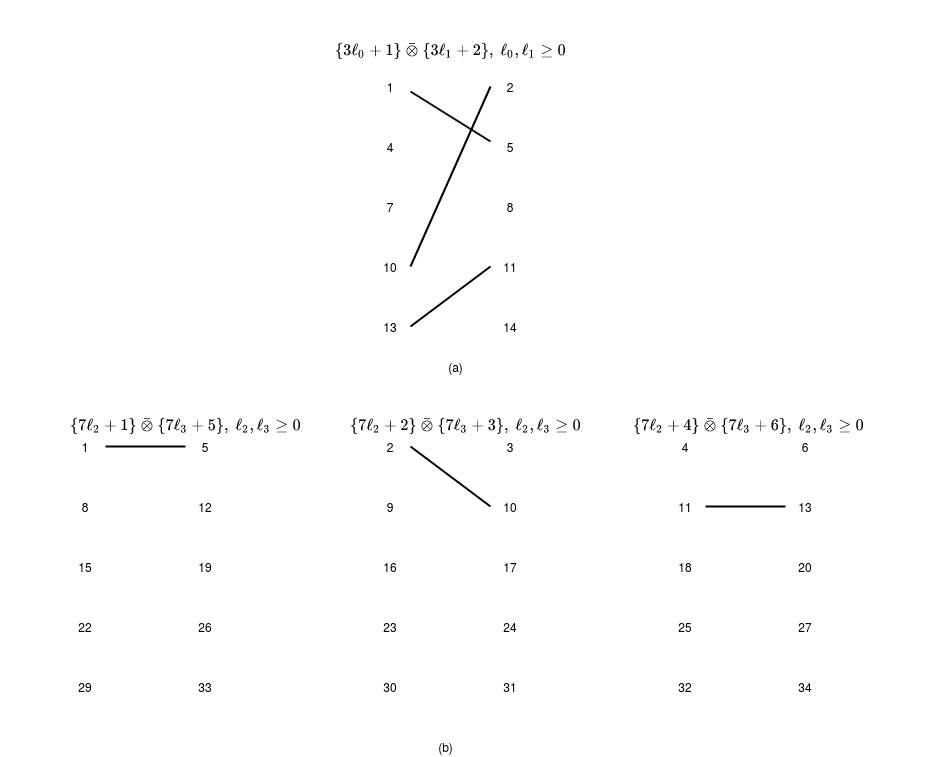
\includegraphics[width=0.45\textwidth]{./ConfSources/pair_union.png}
%		\caption{Visual representation of $(\alpha,~\beta)$ }
%		\label{fig:example5-union}
%		\end{figure}
\label{ex-5}
\end{example}
 








\section{validity confirmation through the Union Bound}
\label{sec4}
%For a given RSC code, the distance spectrum provides information concerning the multiplicity of a codeword for a fixed weight and it is an effective tool to evaluate its error-correcting capability. In practice however, since higher-weight codewords have very little effect on its overall error-correcting capability, we usually use a partial distance spectrum, where the largest codeword weight value is set to $d_{\text{max}}$. 

%The distance spectrum of the RSC code can be obtained from its transfer function, denoted by $$T(Y,X)=\sum_{d=0}^{\infty}\sum_{w=0}^{\infty} a(d,w)Y^dX^w$$ where $a(d,w)$ is the number of codewords of weight $d$ generated by an input bit sequence of weight $w$. 
%The transfer function enumerates all the paths that diverge from and then return to the initial state \cite{ref3}, \textit{i.e.} the RTZ input paths. 
%Once the transfer function of an RSC code is known, it can be used to obtain bounds on the error-correcting capability using the union bound.
%Unfortunately, the complexity involved in deriving the transfer function increases as the number of states of the RSC code increases and other methods such as Mason's Rule \cite{ref3} have to be used. 

%For a given RSC code, we have shown in \ref{subsec:low-weight} that each codeword $c(x)$ is made up of $b(x)$ and $h(x)$ which have $a(x)$ as their common factor as shown in (\ref{novelEq2}) and (\ref{novelEq3}).
 In this section, we obtain a union bound using the low-weight codeword components pattern list and compare it to the union bound obtained via the transfer function as well as simulation results in order to confirm the validity of our proposed method.

\subsection{A novel union bound}
To obtain a union bound, let $\cA_h(d)$ be the set of all $a(x)$ which yields weight-$d$ PCs \ie, $w_H(h(x))=w_H(a(x)f(x))=d$ for $a(x) \in \cA_h(d)$. Similarly, we also define $\cA_b(d)$ and $\cA_c(d)$ for weight-$d$ SCs and codewords, respectively, in the same manner.

Then, for $w_H(b(x)), w_H(h(x)) \geq 2$, we have from \eqref{eq:cw-weight} that
\begin{align}
\cA_c(d) = \bigcup_{\ell = 2}^{d-2} \left\{\cA_b(\ell) \cap \cA_h(d-\ell)\right\}
\label{Eq:exactset}
\end{align}
However, to determine $\cA_b(\ell)$ or $\cA_h(\ell)$ for a large $\ell$ is a complex task in general. Thus, in this paper, we replace the set $\cA_c(d)$ by the following approximated set %\eqref{setApprox}
\begin{equation}
\begin{split}
\cA_c(d) \approx \cA_c'(d) &= \left\{\bigcup_{\ell = 2}^{\ell+1} \left\{\cA_b(\ell) \cap \cA_h(d-\ell)\right\}\right\}\bigcup \left\{\bigcup_{\ell = 2}^{\ell+1} \left\{\cA_b(d-\ell) \cap \cA_h(\ell)\right\}\right\}
\end{split}
\label{setApprox}
\end{equation}
where some codewords in $\cA_c(d)$ with $\ell \approx d-\ell$ may be ignored in $\cA_c'(d)$.
Finally, we obtain the following union bound
\begin{align}
P_b \leq \frac{1}{k} \sum_{d=d_{\text{free}}}^{d_{\text{max}}} \sum_{a(x) \in \cA'_c(d)}w_H(a(x)g(x)) Q\Bigg( \sqrt{\frac{2dE_c}{N_0}}\Bigg)
\label{novelEq7}
\end{align}
where we let $d_{\text{max}}=d_{\text{free}}+3$. 

In order to determine the low-weight codewords, based on $f(x)$, we first generate $\cA_h(2)\cup\cA_h(3)$, the set consisting of the weight-2 and -3 PCs (if they exist) using our proposed method described in the previous section. After that, we obtain the set consisting of SCs $b(x)=a(x)g(x)$ for $a(x) \in \cA_h(2)\cup\cA_h(3)$. Similarly, based on $g(x)$, we also obtain the set consisting of $h(x)=a(x)f(x)$ for $a(x) \in \cA_s(2)\cup\cA_s(3)$. Then, the resulting table consists of SCs and PCs such that $w_H(b(x))+w_H(h(x)) \leq d_{\text{max}}$.

\begin{example} {5/7 RSC code $\left(f(x)=1+x^2,~g(x)=1+x+x^2\right)$}
	
	The characteristics of $f(x)$ as well as the low-weight PCs it generates are shown in Example \ref{ex-3}  whiles the characteristics of $g(x)$ as well as the low-weight SCs are shown in  Example \ref{ex-1}. The SCs and PCs of the 5/7 RSC code are listed in Table \ref{novelTab13}. 
	\begin{table}[htbp]
		\caption{SCs and PCs for the $5/7$ RSC code}
		\centering
		\begin{tabularx}{0.75\textwidth}{Xlll} 
			\toprule
			$w_H(c(x))$& $a(x)$ & $b(x)$ & $h(x)$ \\ %[0.5ex] 
			\midrule
			5&$1$ & $1+x+x^{2}$ & $1+x^2$\\
			\hline
			6&$1+x$ & $1+x^3$ & $1+x+x^2+x^3$\\
			&$1+x^2$ & $1+x+x^3+x^4$ & $1+x^{4}$\\
			\hline
			&$1+x+x^2$ & $1+x^2+x^4$ & $1+x+x^3+x^4$\\
			%\hline
			&$1+x+x^3$ & $1+x^4+x^5$ & $1+x+x^2+x^5$\\
			7&$1+x^2+x^3$ & $1+x+x^5$ & $1+x^3+x^4+x^5$\\
			&$1+x^2+x^4$ & $1+x+x^3+x^5+x^6$ & $1+x^{6}$\\			
			\hline
			8&$1+x+x^3+x^4$ & $1+x^6$ & $1+x+x^2+x^4+x^5+x^6$\\
			&$1+x^2+x^4+x^6$ & $1+x+x^3+x^5+x^7+x^8$ & $1+x^8$\\
			%\hline
			
			\bottomrule
			%======extra
			%\hline
			%$1+x+x^3+x^5$ & $1+x^4+x^6+x^7$ & $1+x+x^2+x^7$\\
			%\hline
			%$1+x+x^2+x^4$ & $1+x^2+x^5+x^6$ & $1+x+x^3+x^6$\\
			%\hline
			%$1+x+x^2+x^3$ & $1+x^2+x^3+x^5$ & $1+x+x^4+x^5$\\
			%\hline
			%$1+x^2+x^3+x^5$ & $1+x+x^6+x^7$ & $1+x^3+x^4+x^7$\\
			%\hline
			%$1+x^2+x^3+x^4$ & $1+x+x^4+x^6$ & $1+x^3+x^5+x^6$\\
			%\hline
			%$1+x^2+x^4+x^5$ & $1+x+x^3+x^7$ & $1+x^5+x^6+x^7$\\
		\end{tabularx}
		
		\label{novelTab13}
	\end{table}
\end{example}

\begin{example}{37/21 RSC code $\left( f(x)=1+x+x^2+x^3+x^4 , ~g(x)=1+x^4\right)$}
	
	The  SCs and PCs for this RSC code are listed in Table \ref{novelTab14}.
	The low-weight SCs and PCs were obtained using the methods in Examples \ref{ex-3} and \ref{ex-2}, respectively. 
	\begin{table}[htbp]
		\caption{SCs and PCs for the $37/21$ RSC code}
		\centering
		\begin{tabularx}{0.75\textwidth}{Xlll} 
			\toprule
			$w_H(c(x))$&$a(x)$ & $b(x)$ & $h(x)$ \\ [0.5ex] 
			\midrule
			6&$1+x$ & $1+x+x^{4}+x^5$ & $1+x^5$\\
			\hline
			7&$1$ & $1+x^4$ & $1+x+x^2+x^3+x^4$\\
			\hline
			8&$1+x+x^5+x^6$ & $1+x+x^4+x^6+x^9+x^{10}$ & $1+x^{10}$\\
			\bottomrule
			%$1+x+x^4+x^5$ & $1+x+x^8+x^9$ & $1+x^4+x^5+x^9$\\
			%\hline
			%$1+x^2$ & $1+x^2+x^4+x^6$ & $1+x+x^5+x^6$\\
			%\hline
			%$1+x+x^5$ & $1+x+x^4+x^9$ & $1+x^6+x^7+x^8+x^9$\\
			%\hline
			%$1+x+x^4$ & $1+x+x^5+x^8$ & $1+x^4+x^6+x^7+x^8$\\
			%\hline
			%$1+x^2+x^4$ & $1+x^2+x^6+x^8$ & $1+x+x^4+x^7+x^8$\\
			%\hline
			%$1+x^3+x^4$& $1+x^3+x^7+x^8$ & $1+x+x^2+x^4+x^8$\\
			%\hline
			%$1+x^4+x^5$ & $1+x^5+x^8+x^9$ & $1+x+x^2+x^3+x^9$\\
		\end{tabularx}
		
		\label{novelTab14}
	\end{table}
	\label{ex-7}
\end{example}

\begin{example}{$23/35$ RSC code $\left(f(x)=1+x+x^4,~g(x)=1+x^2+x^3+x^4 \right)$}
	
	Using the procedure shown in Examples  \ref{ex-1} and  \ref{ex-5}, we obtained the  low-weight PCs and SCs, respectively.
	The corresponding SCs and PCs  for the 23/35 RSC code are listed Table \ref{novelTab14}.
	\begin{table}[htbp]
		\caption{SCs and PCs for the $23/35$ RSC code}
		\centering
		\begin{tabularx}{0.75\textwidth}{lXlX} 
			\toprule
			$w_H(c(x))$ & $a(x)$ & $b(x)$ & $h(x)$ \\ [0.5ex] 
			\midrule
			7&$1$ & $1+x^2+x^3+x^4$ & $1+x+x^{4}$\\
			\hline
			&$1+x^2+x^3$ & $1+x^7$ & $1+x+x^2+x^6+x^7$\\
			\hline 
			9&$1+x+x^2+x^3+x^5$ & $1+x+x^3+x^4+x^8+x^9$ & $1+x^7+x^9$\\
			\hline
			&$1+x+x^2+x^3+x^5+x^7+x^8$ & $1+x+x^3+x^4+x^7+x^{12}$ & $1+x^{11}+x^{12}$\\
			\hline
			10&$1+x^2+x^3+x^7+x^9+x^{10}$ & $1+x^{14}$ & $1+x+x^2+x^6+x^8+x^9+x^{13}+x^{14}$\\
			\bottomrule
		\end{tabularx}
		
		\label{novelTab15}
	\end{table}
\end{example}

\subsection{Numerical results}
We verify the validity of our proposed method for the $5/7,~37/21$ and $23/35$ RSC codes, assuming a frame size of $N=64$ is used to obtain the simulation results. 
%, we compared the bounds in \eqref{novelEq7} with that obtained using the transfer function method as well as the simulation results for the 
%For each RSC code and a frame size of $N=64$, the codeword is BPSK modulated and transmitted over the AWGN channel. At the receiver end, the Viterbi algorithm is used to decode before a decision is made on the decoded sequence.



From Table \ref{novelTab13}, we observe that every SC such that $w_H(b(x)) >3$ is either a combination of only weight-2 SCs or only weight-3 SCs or both. This means that when the 5/7 RSC code is used in a TC, the deterministic interleaver should be designed in such a way that it deals effectively with both weight-2 and weight-3 SCs. While, having to consider weight-3 SCs in the deterministic interleaver design introduces a bit of complexity, it is manageable since there is just a single $(m,n)$ pair that is associated with the weight-3 SCs.

\begin{figure}[htbp]
	\centering
	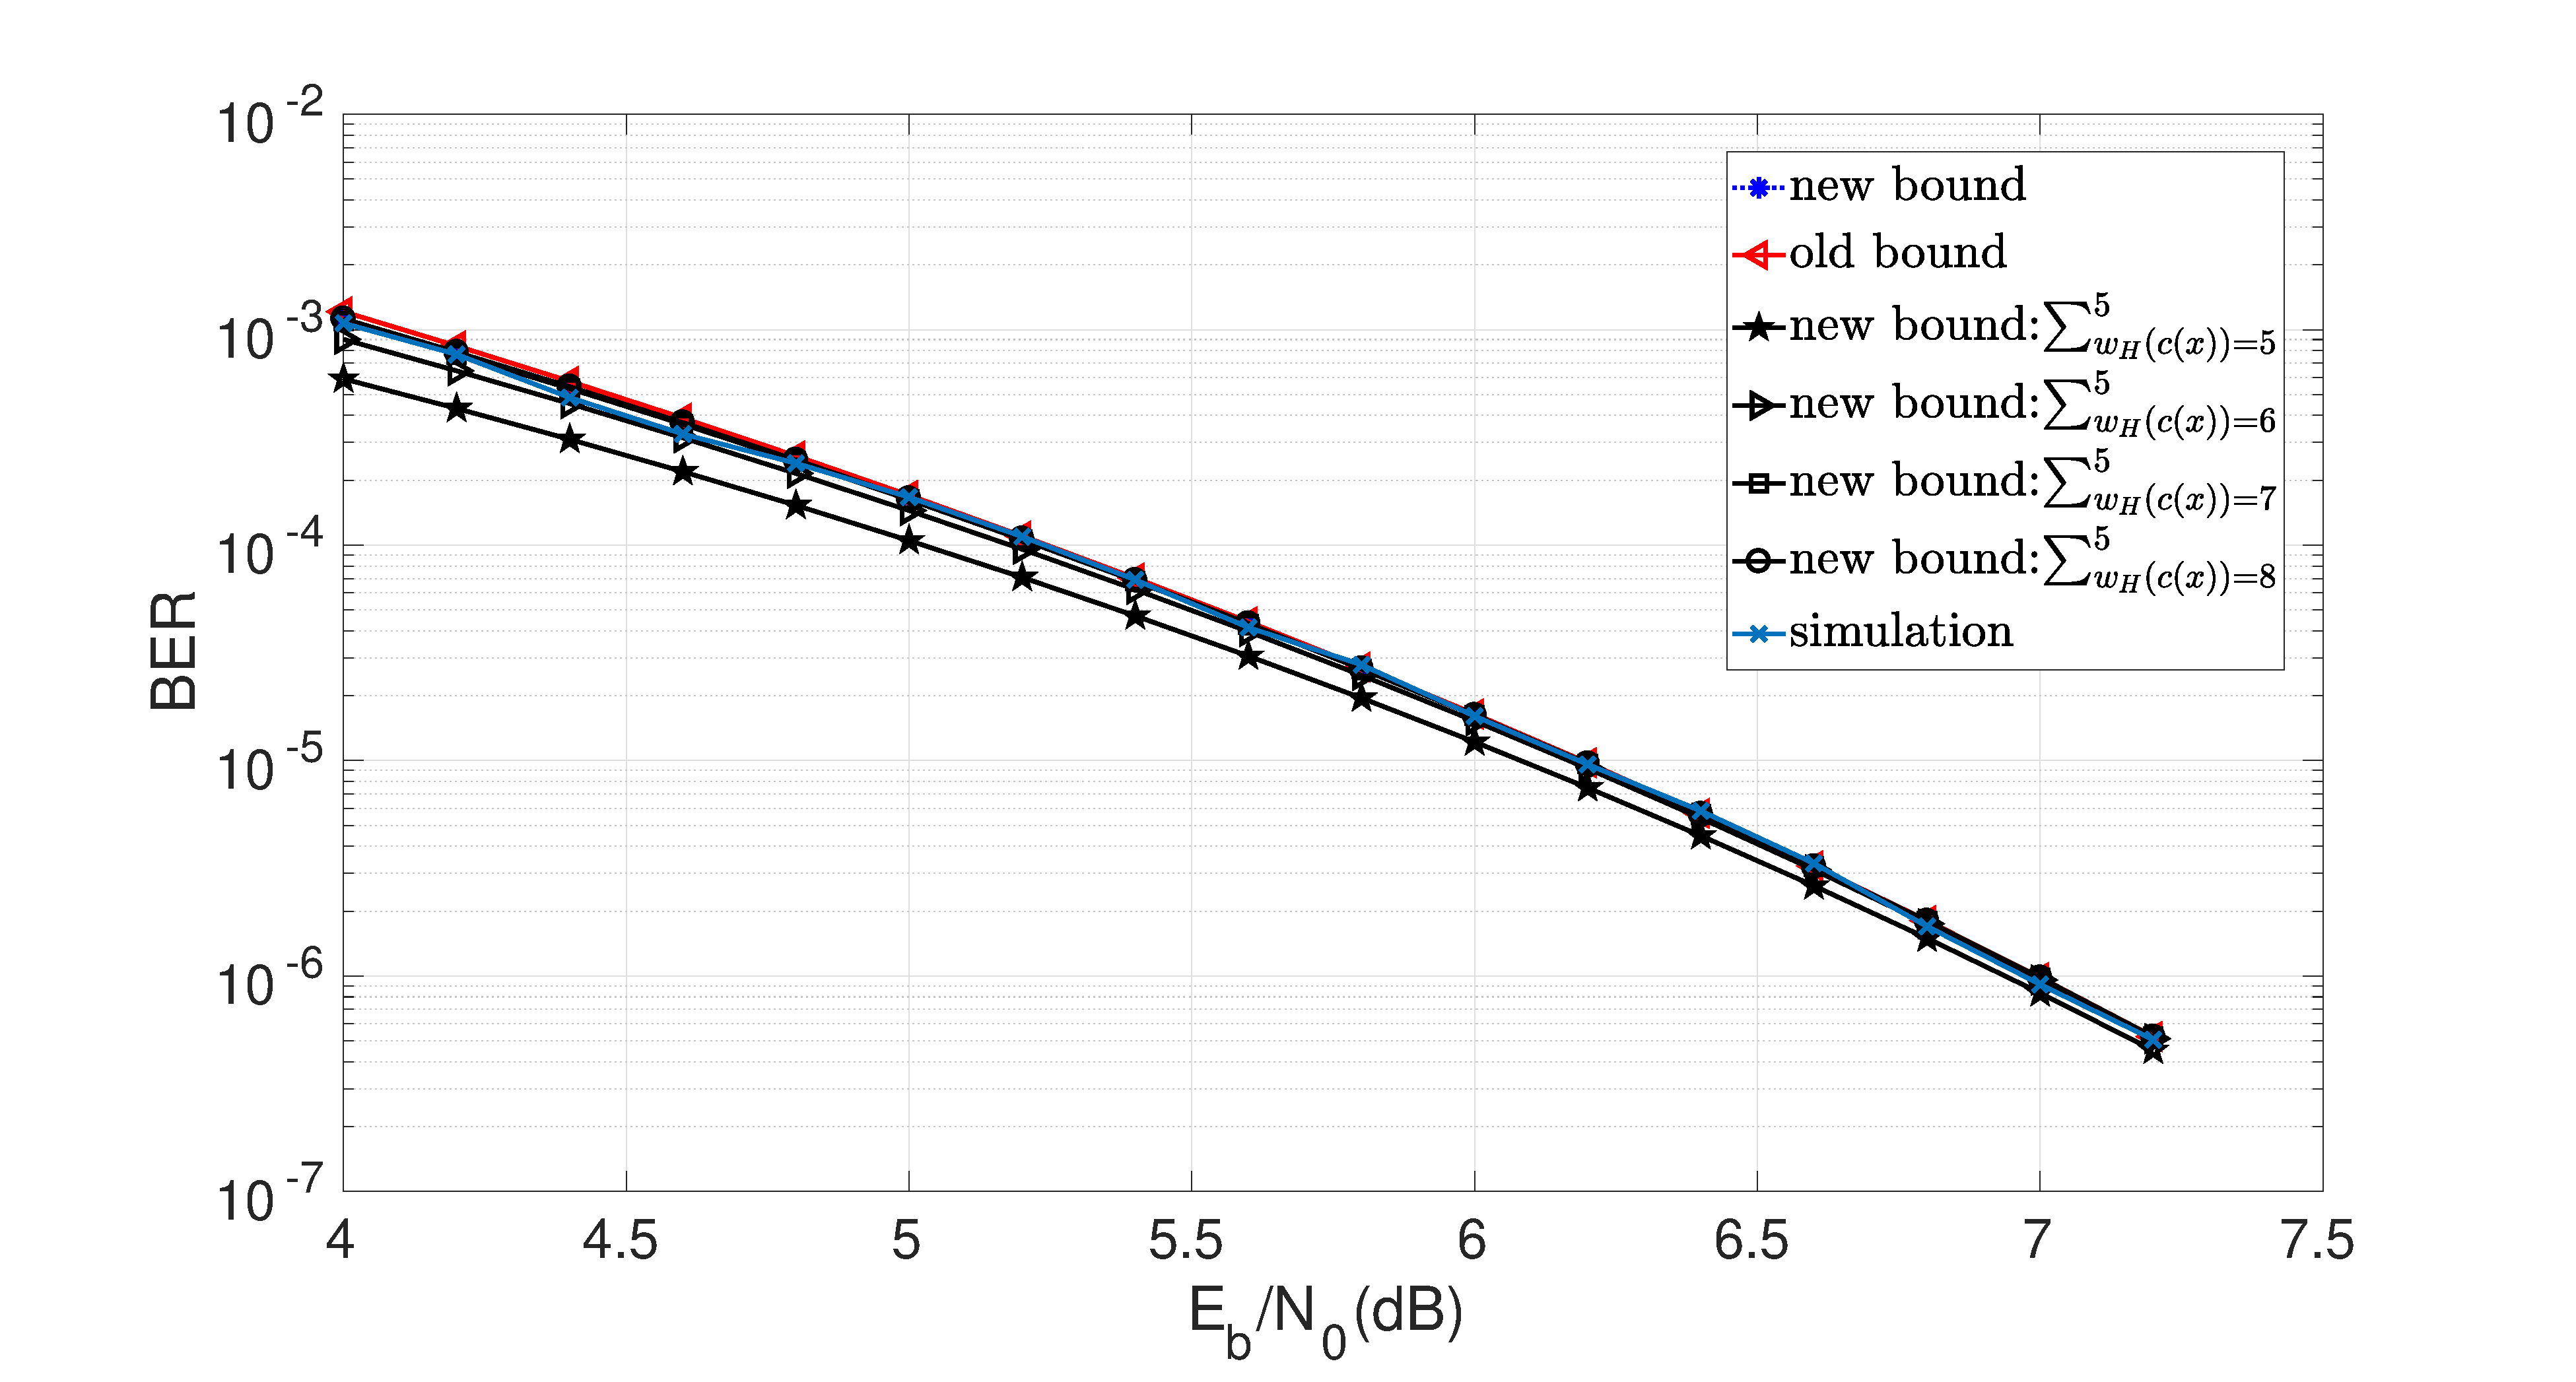
\includegraphics[width=0.5\textwidth]{./Images/RSC_5_7_lower_weights2.eps}
	\captionof{figure}{Old Bound vs New Bound vs Simulation for 5/7 RSC Code}
	\label{simFig1}
\end{figure}

Fig. \ref{simFig1} shows the simulation results for the $5/7$ RSC code as well as the union bound obtained using the transfer function and our proposed method. We can observe that the accuracy of our proposed bound increases with the number of terms used in the approximation. Also, as $E_b/N_0$ increases, the proposed bound as well as the transfer function bound and the simulation results tend to converge. The fact that just a single $(m,n)$ pair needs to be considered for weight-3 SCs during interleaver design makes the 5/7 RSC code attractive for use in TCs.
\label{ex-6}


Table \ref{novelTab14} confirms the non-existence of weight-3 SCs and PCs in the 37/21RSC code, and that every SC such that $w_H(b(x)) > 2$ is a combination of weight-2 SCs. As such, deterministic interleaver design for this RSC code is relatively simpler, since only weight-2 SCs need to be considered.
\begin{figure}[htbp]
	\centering
	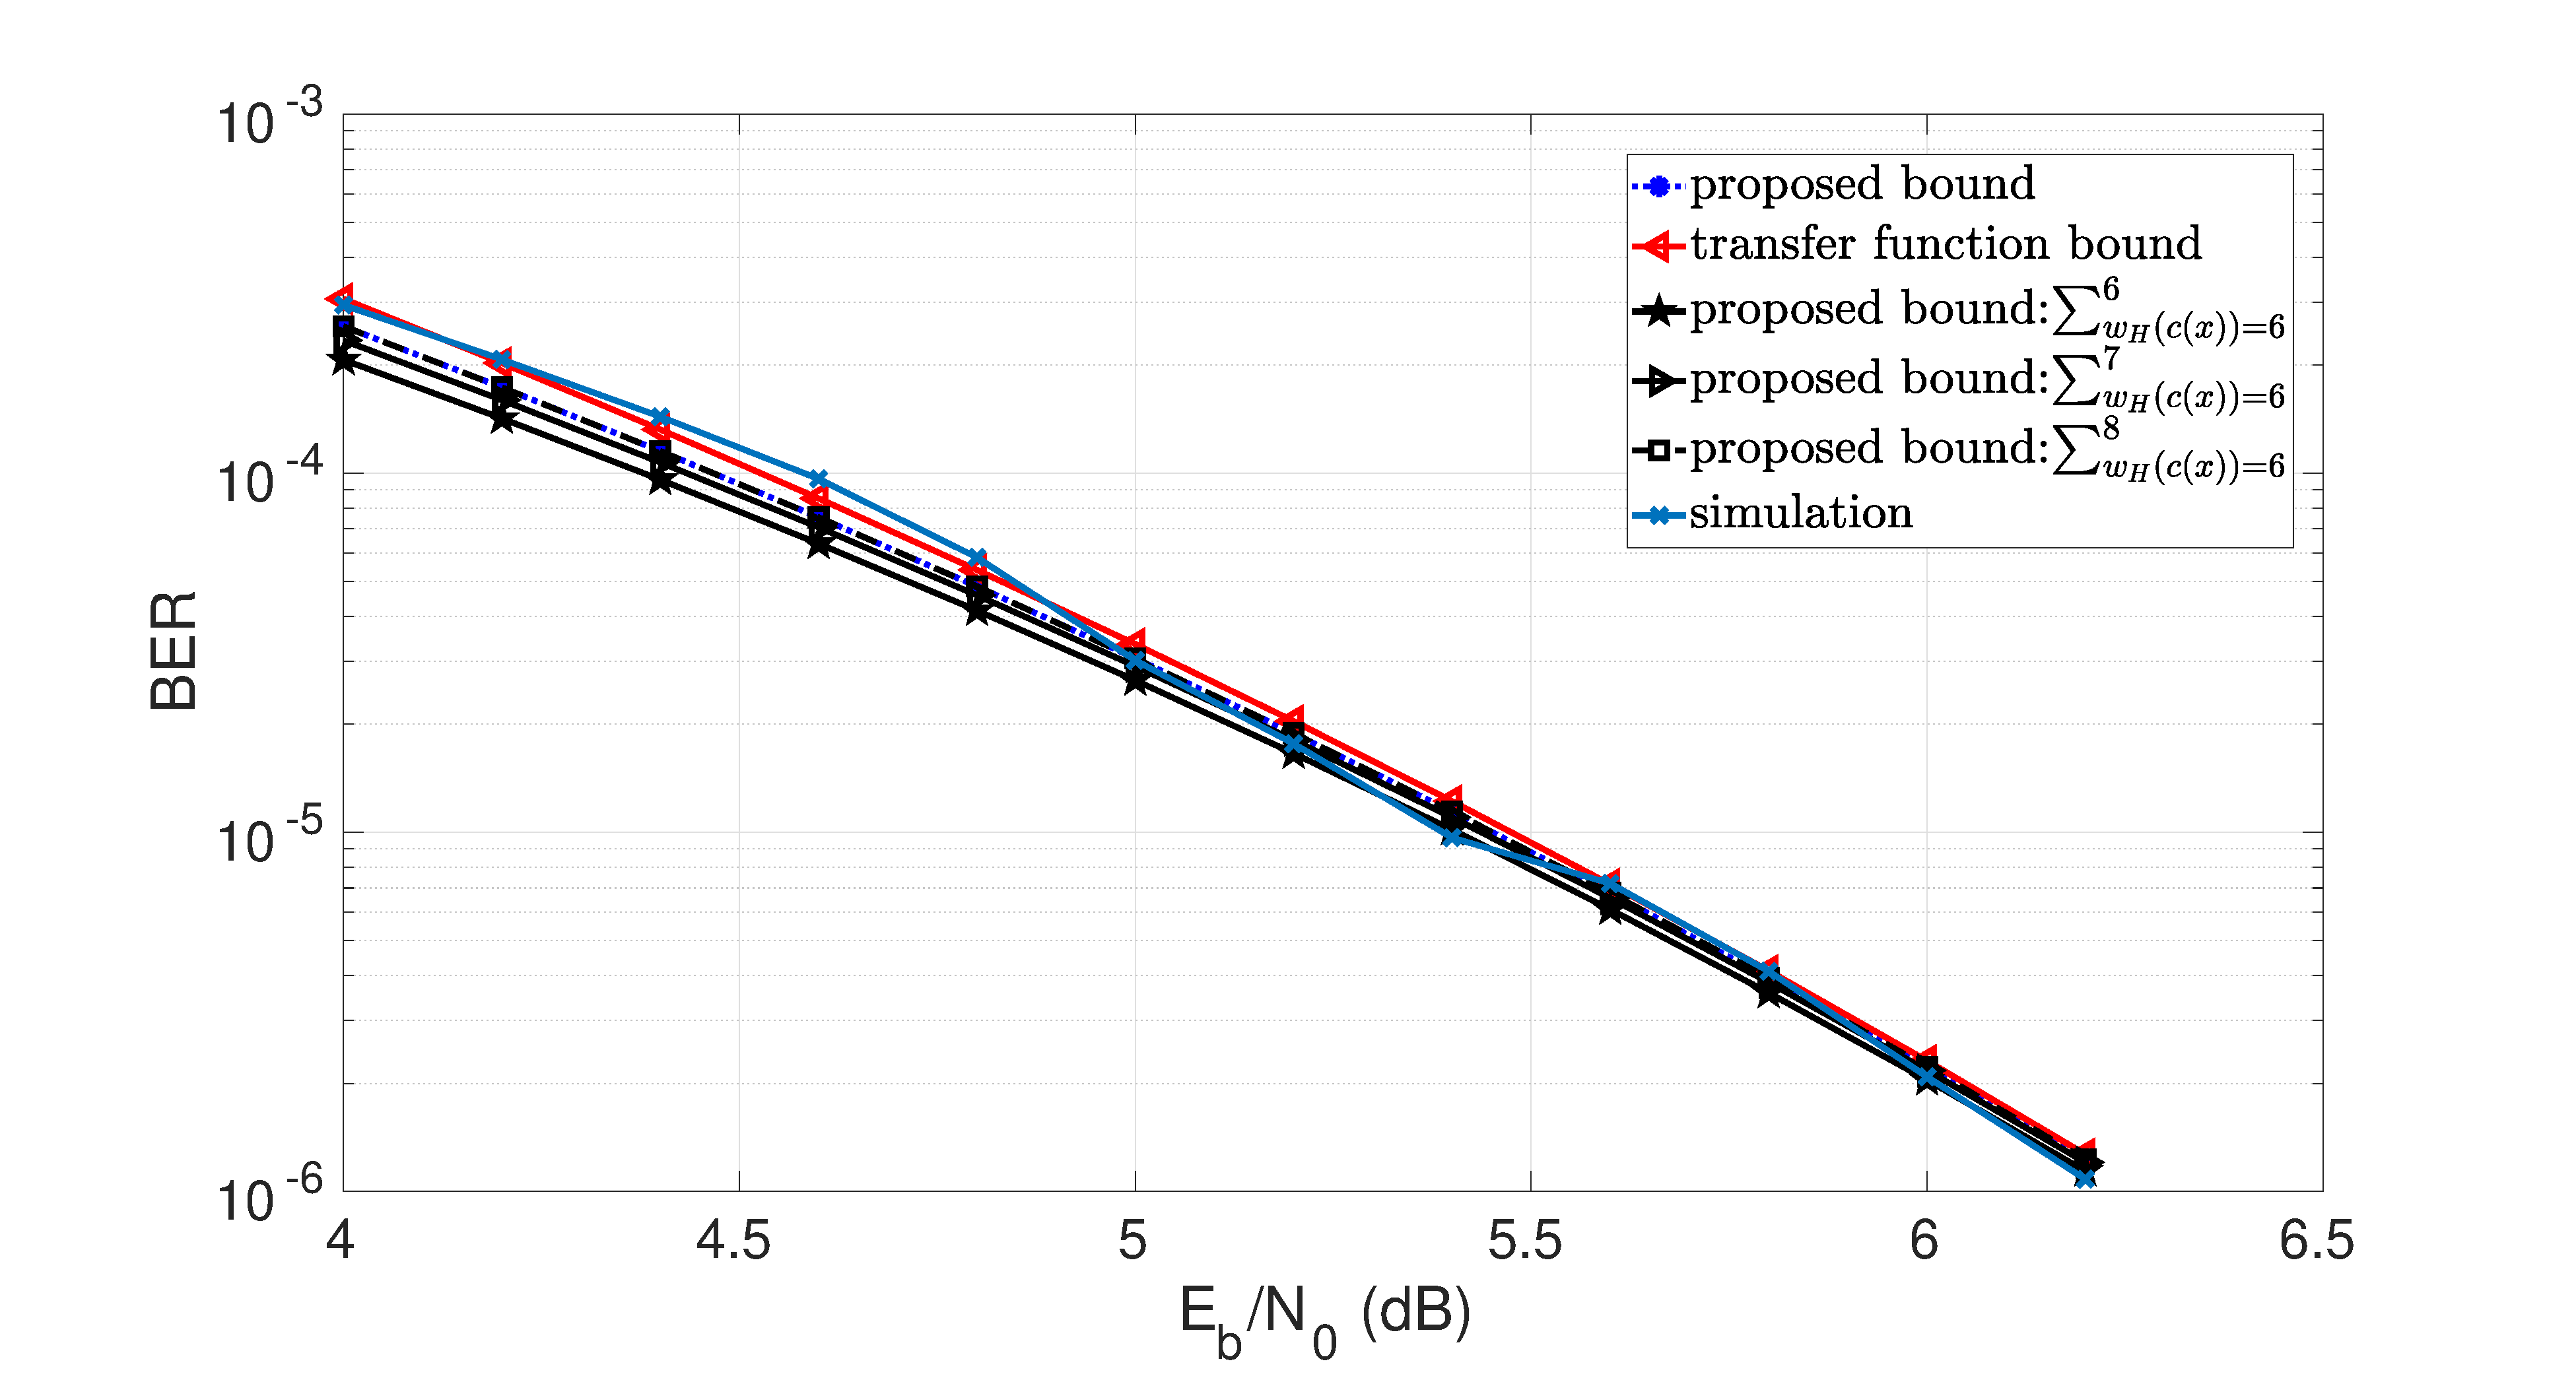
\includegraphics[width=0.5\textwidth]{./Images/RSC_37_21_lower_weights2.eps}
	\caption{Old Bound vs New Bound vs Simulation for 37/21 RSC Code}
	\label{simFig2}
\end{figure}

Simulation results, the transfer function bound and our proposed bound are shown in Fig. \ref{simFig2} for the $37/21$ RSC code. By observation, we can draw conclusions similar to  Example \ref{ex-6} with respect to the accuracy of our proposed bound . Given that weight-2 SCs and PCs are sufficient to derive the union bound, and deterministic interleaver design requires focusing on weight-2 SCs only, this RSC code is highly recommended for use in TCs.

From Table \ref{novelTab15}, we observe that there are no weight-3 SCs. However, there exists weight-4 SCs that are not a combination of weight-2 SCs and when this RSC code is used in TCs, the deterministic interleaver needs to be designed to cater for weight-2 SCs as well as such weight-4 SCs. 
 
\begin{figure}[htbp]
	\centering
	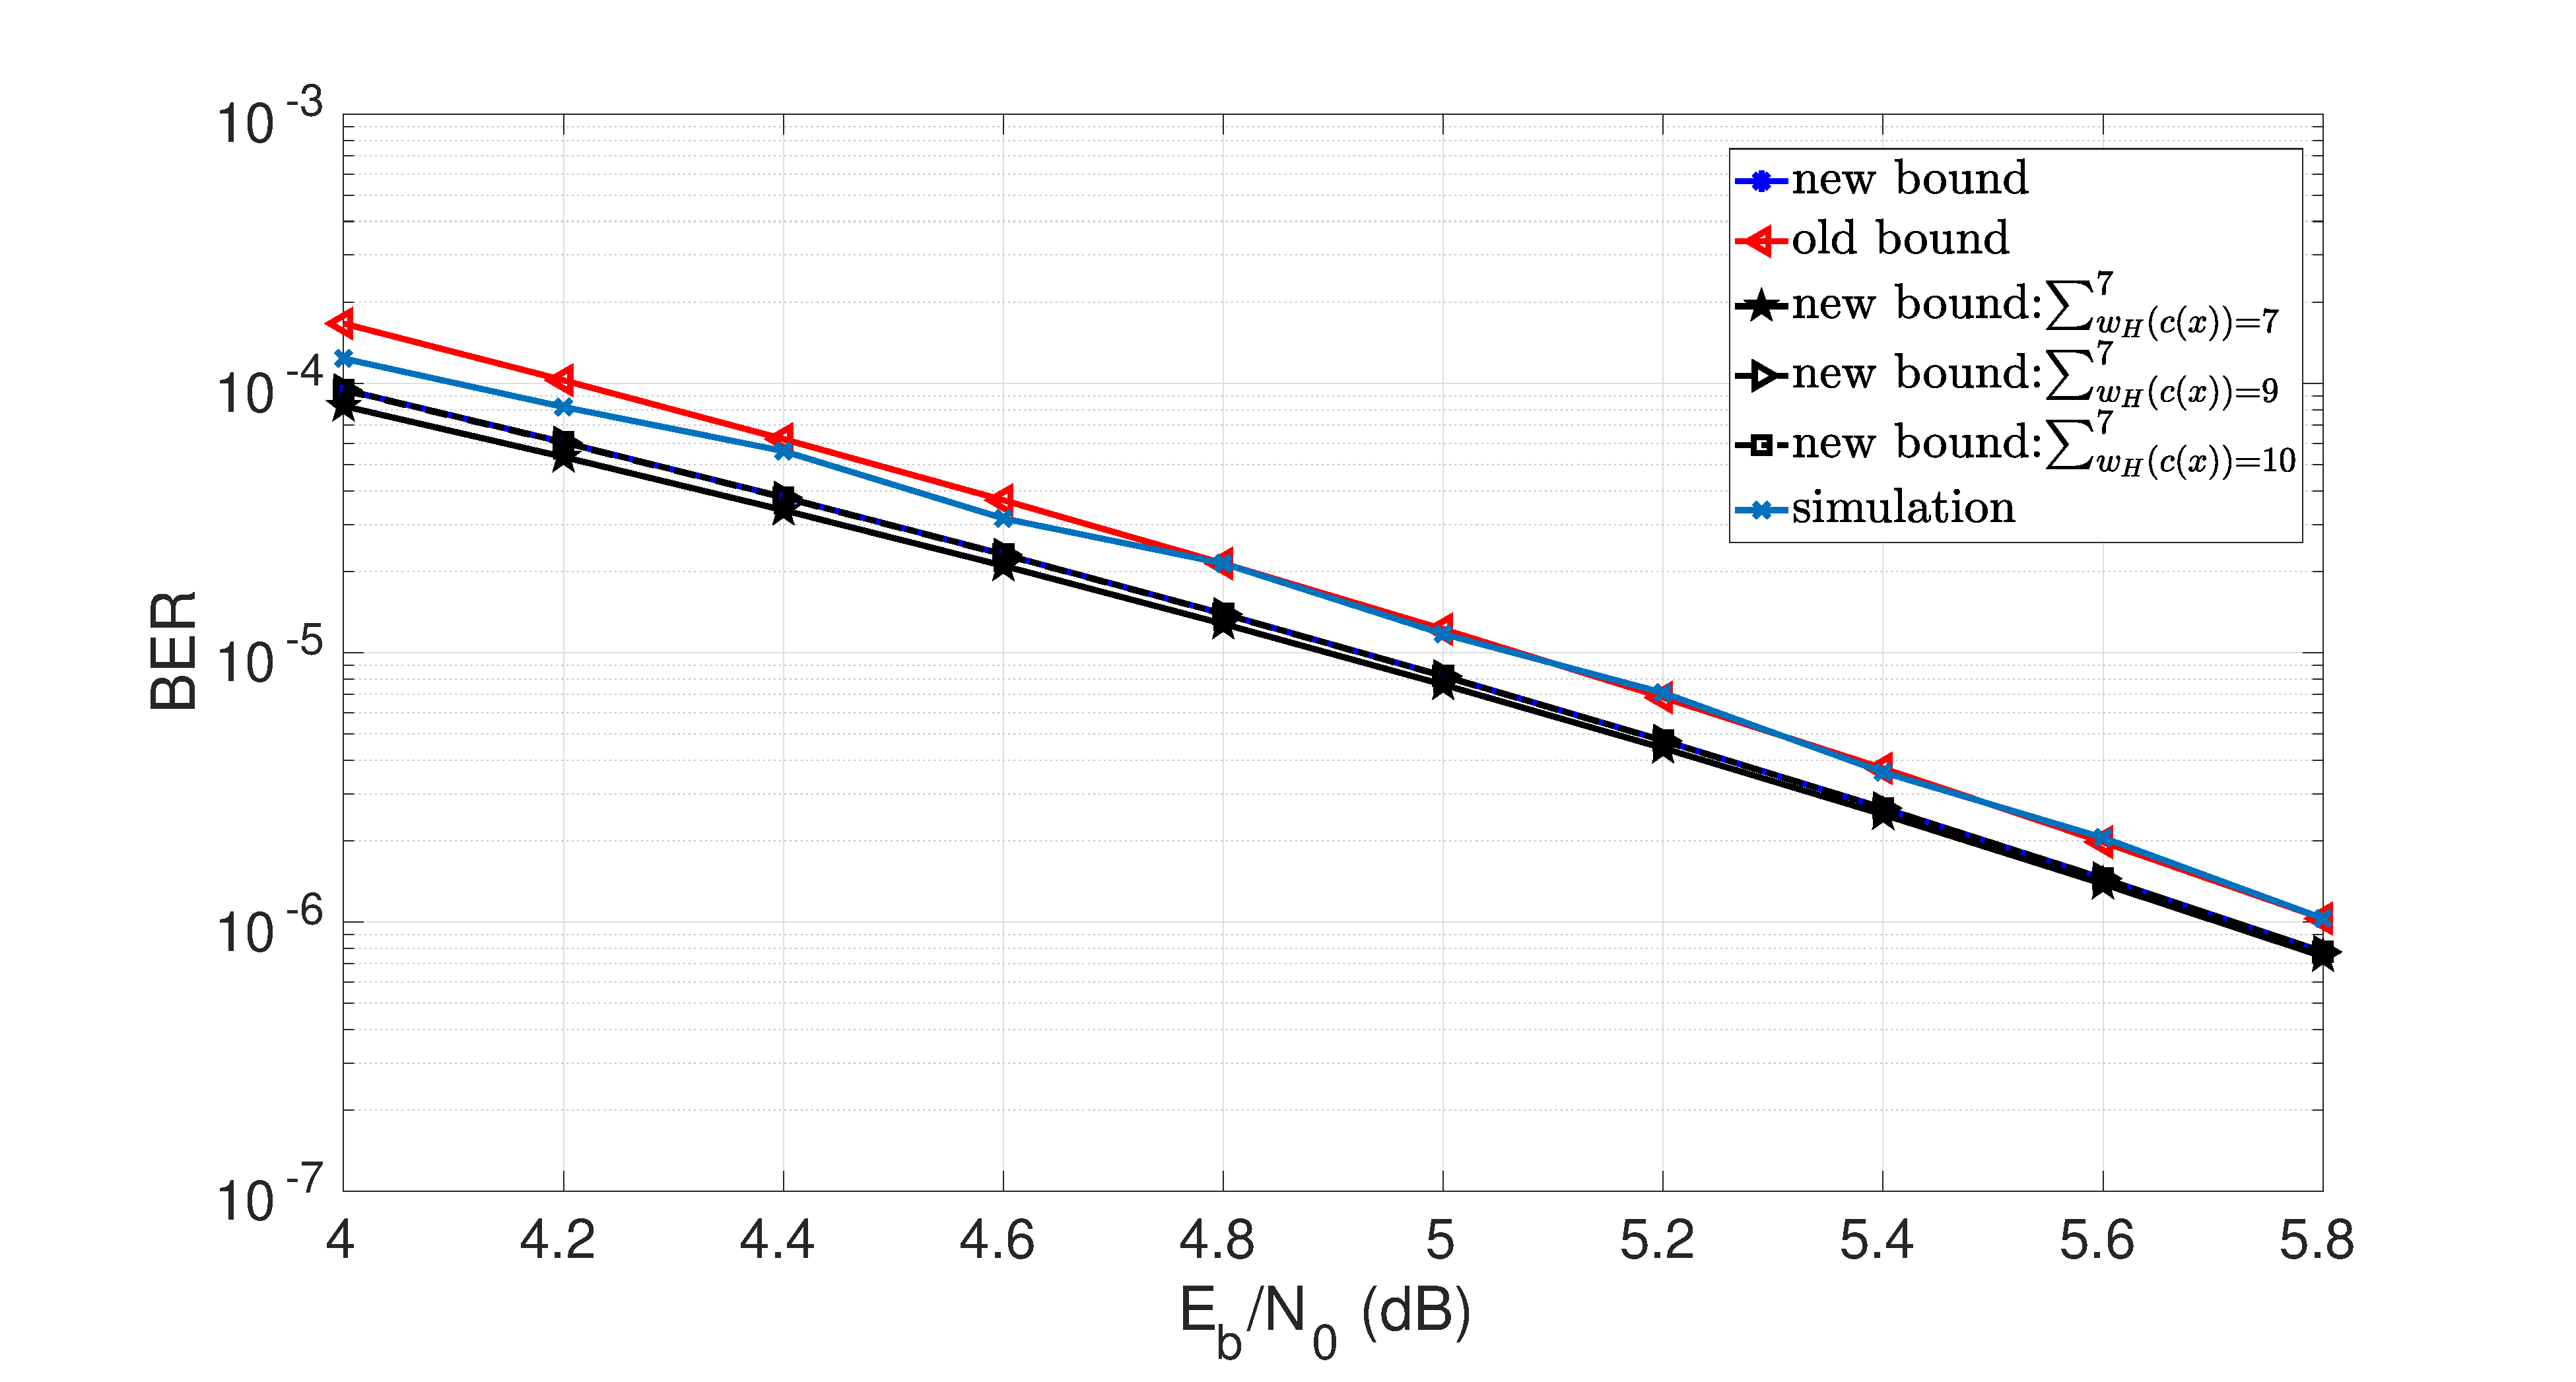
\includegraphics[width=0.5\textwidth]{./Images/RSC_23_35_lower_weights2.eps}
	\caption{Old Bound vs New Bound vs Simulation for 23/35 RSC Code}
	\label{simFig3}
\end{figure}
Fig. \ref{simFig3} shows the simulation results for the $23/35$ RSC code as well as the union bounds obtained using the transfer function as well as our proposed method. Even though the accuracy of our proposed bound increases with the number of terms use, it neither converges with the transfer function bound nor the simulation results as $E_b/N_0$ increases. Even though it is possible to improve the accuracy of our proposed bound by considering SCs and PCs of weight-4, the added complexity as a result of considering weight-4 SCs in the interleaver design process makes this RSC code very unattractive for use in TCs. 


%\begin{figure}[h!]
%\centering
%		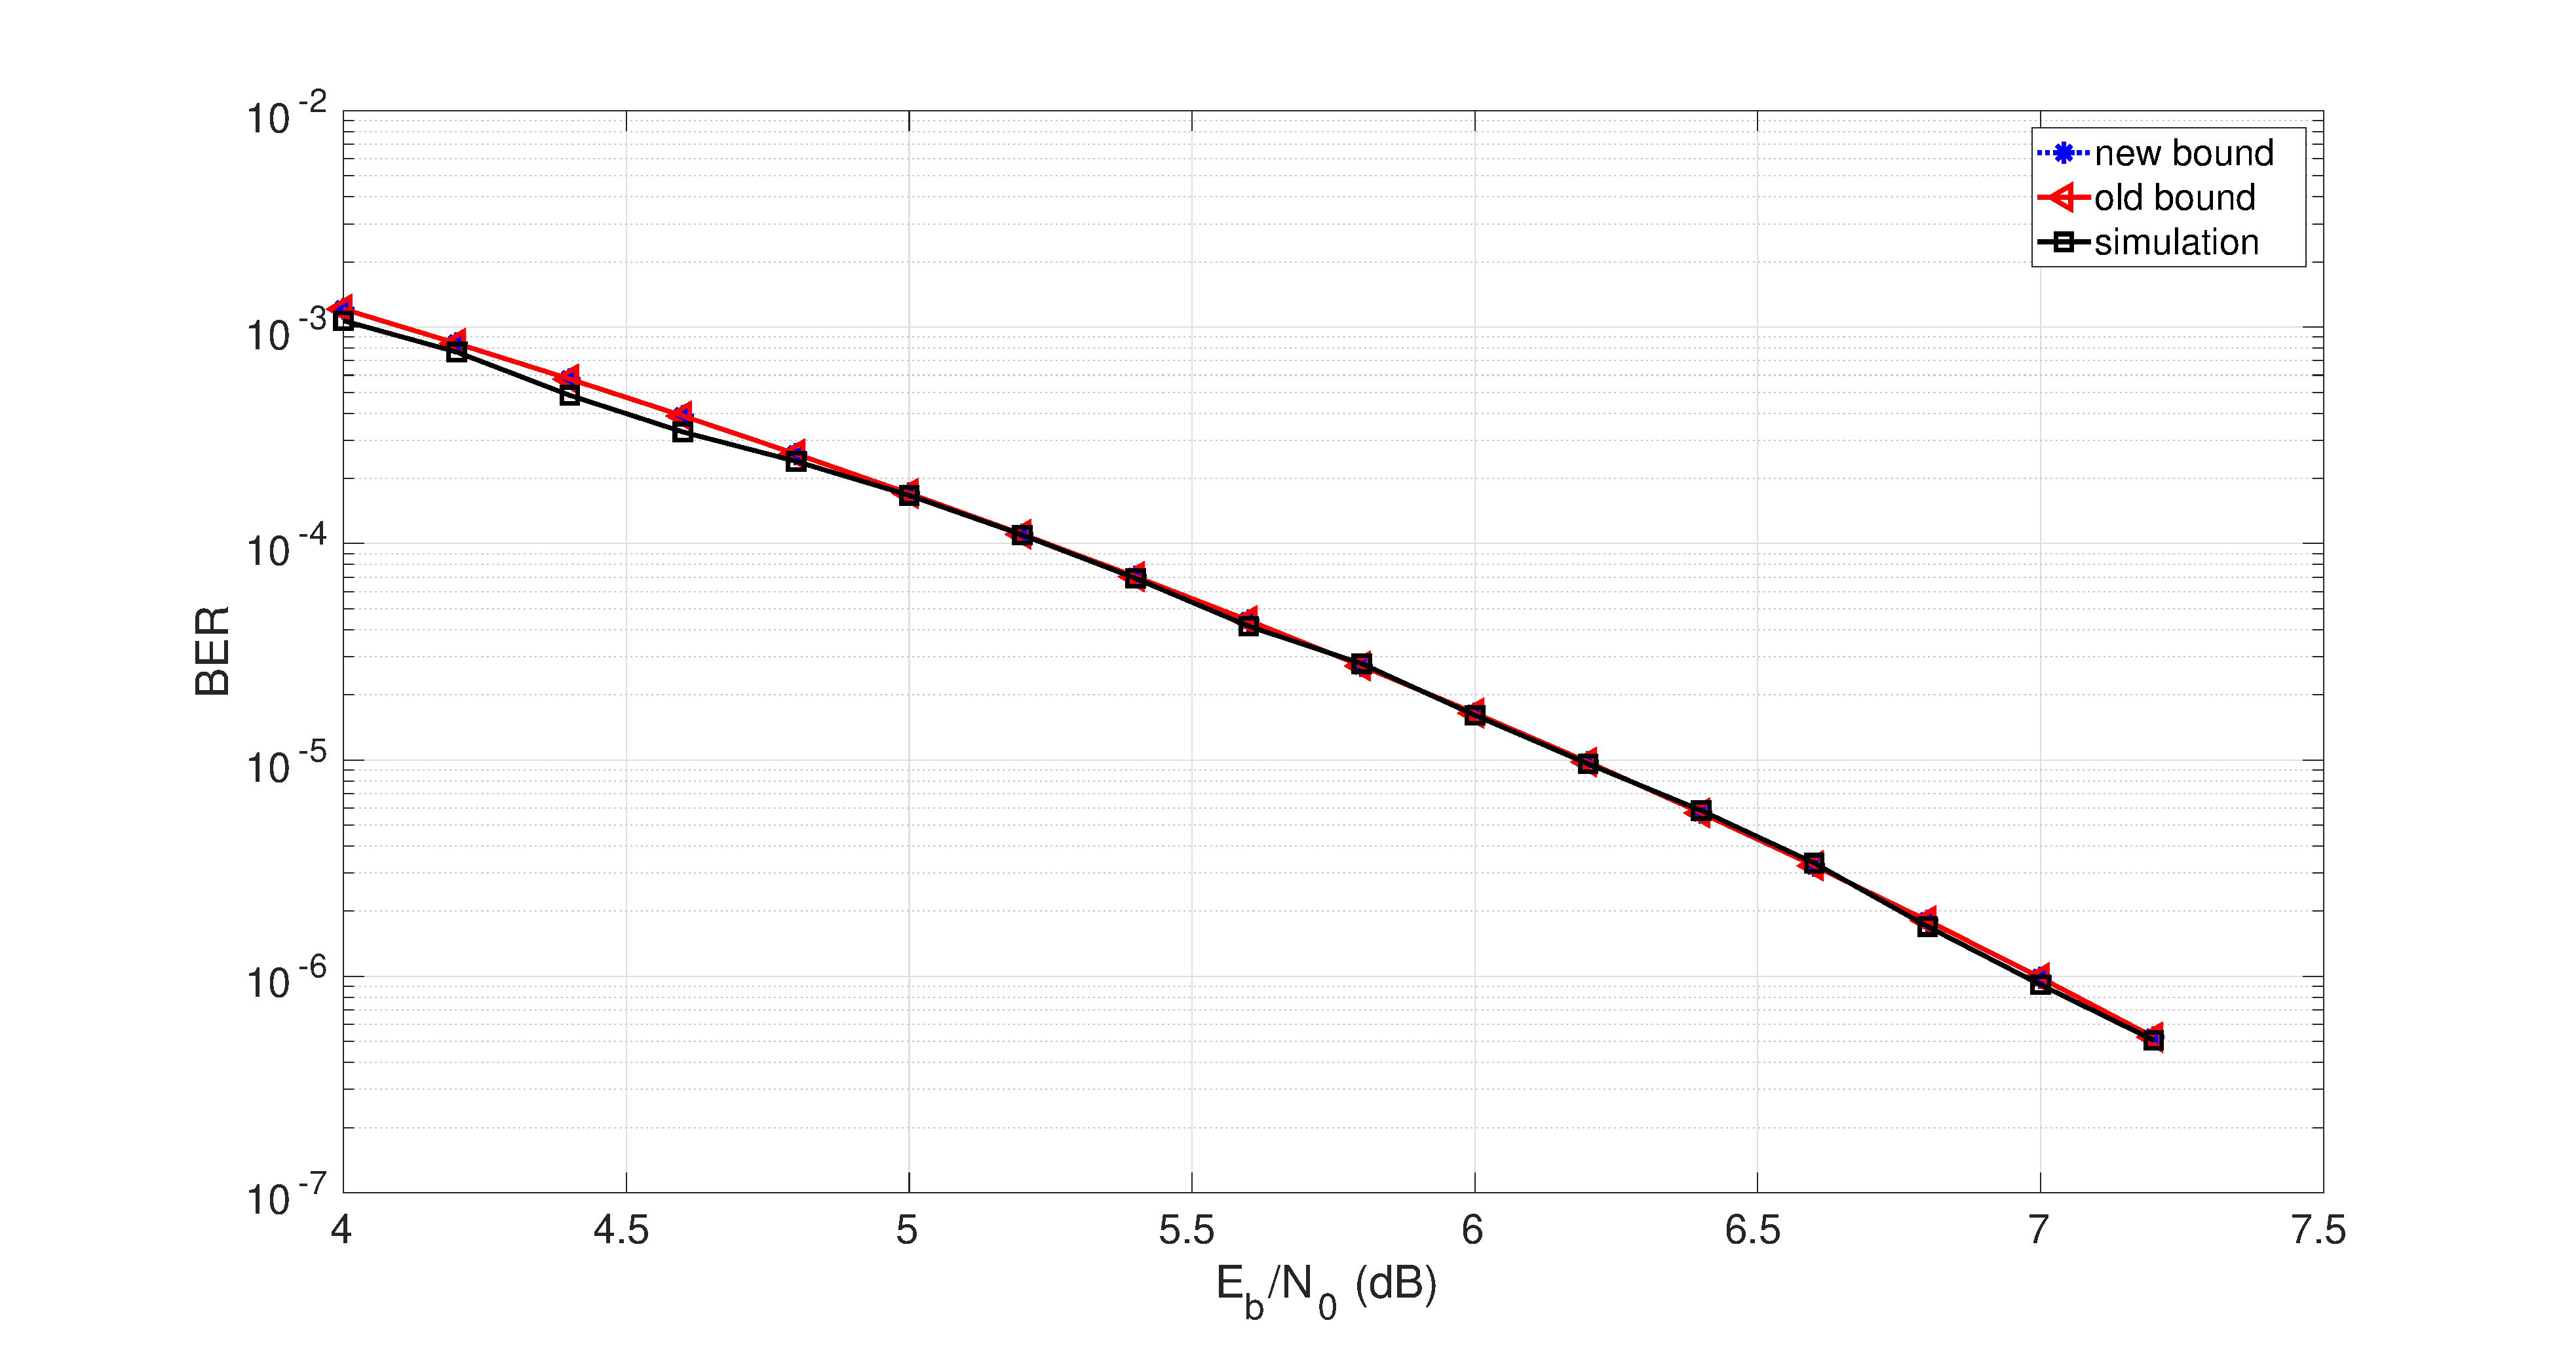
\includegraphics[width=0.8\textwidth]{./Images/RSC_5_7_higher_weights.eps}
%		\caption{Old Bound vs New Bound vs Simulation for 5/7 RSC Code, with higher weights }
%		\label{simFig4}
%		\end{figure}


%		\begin{figure}[h!]
%\centering
%	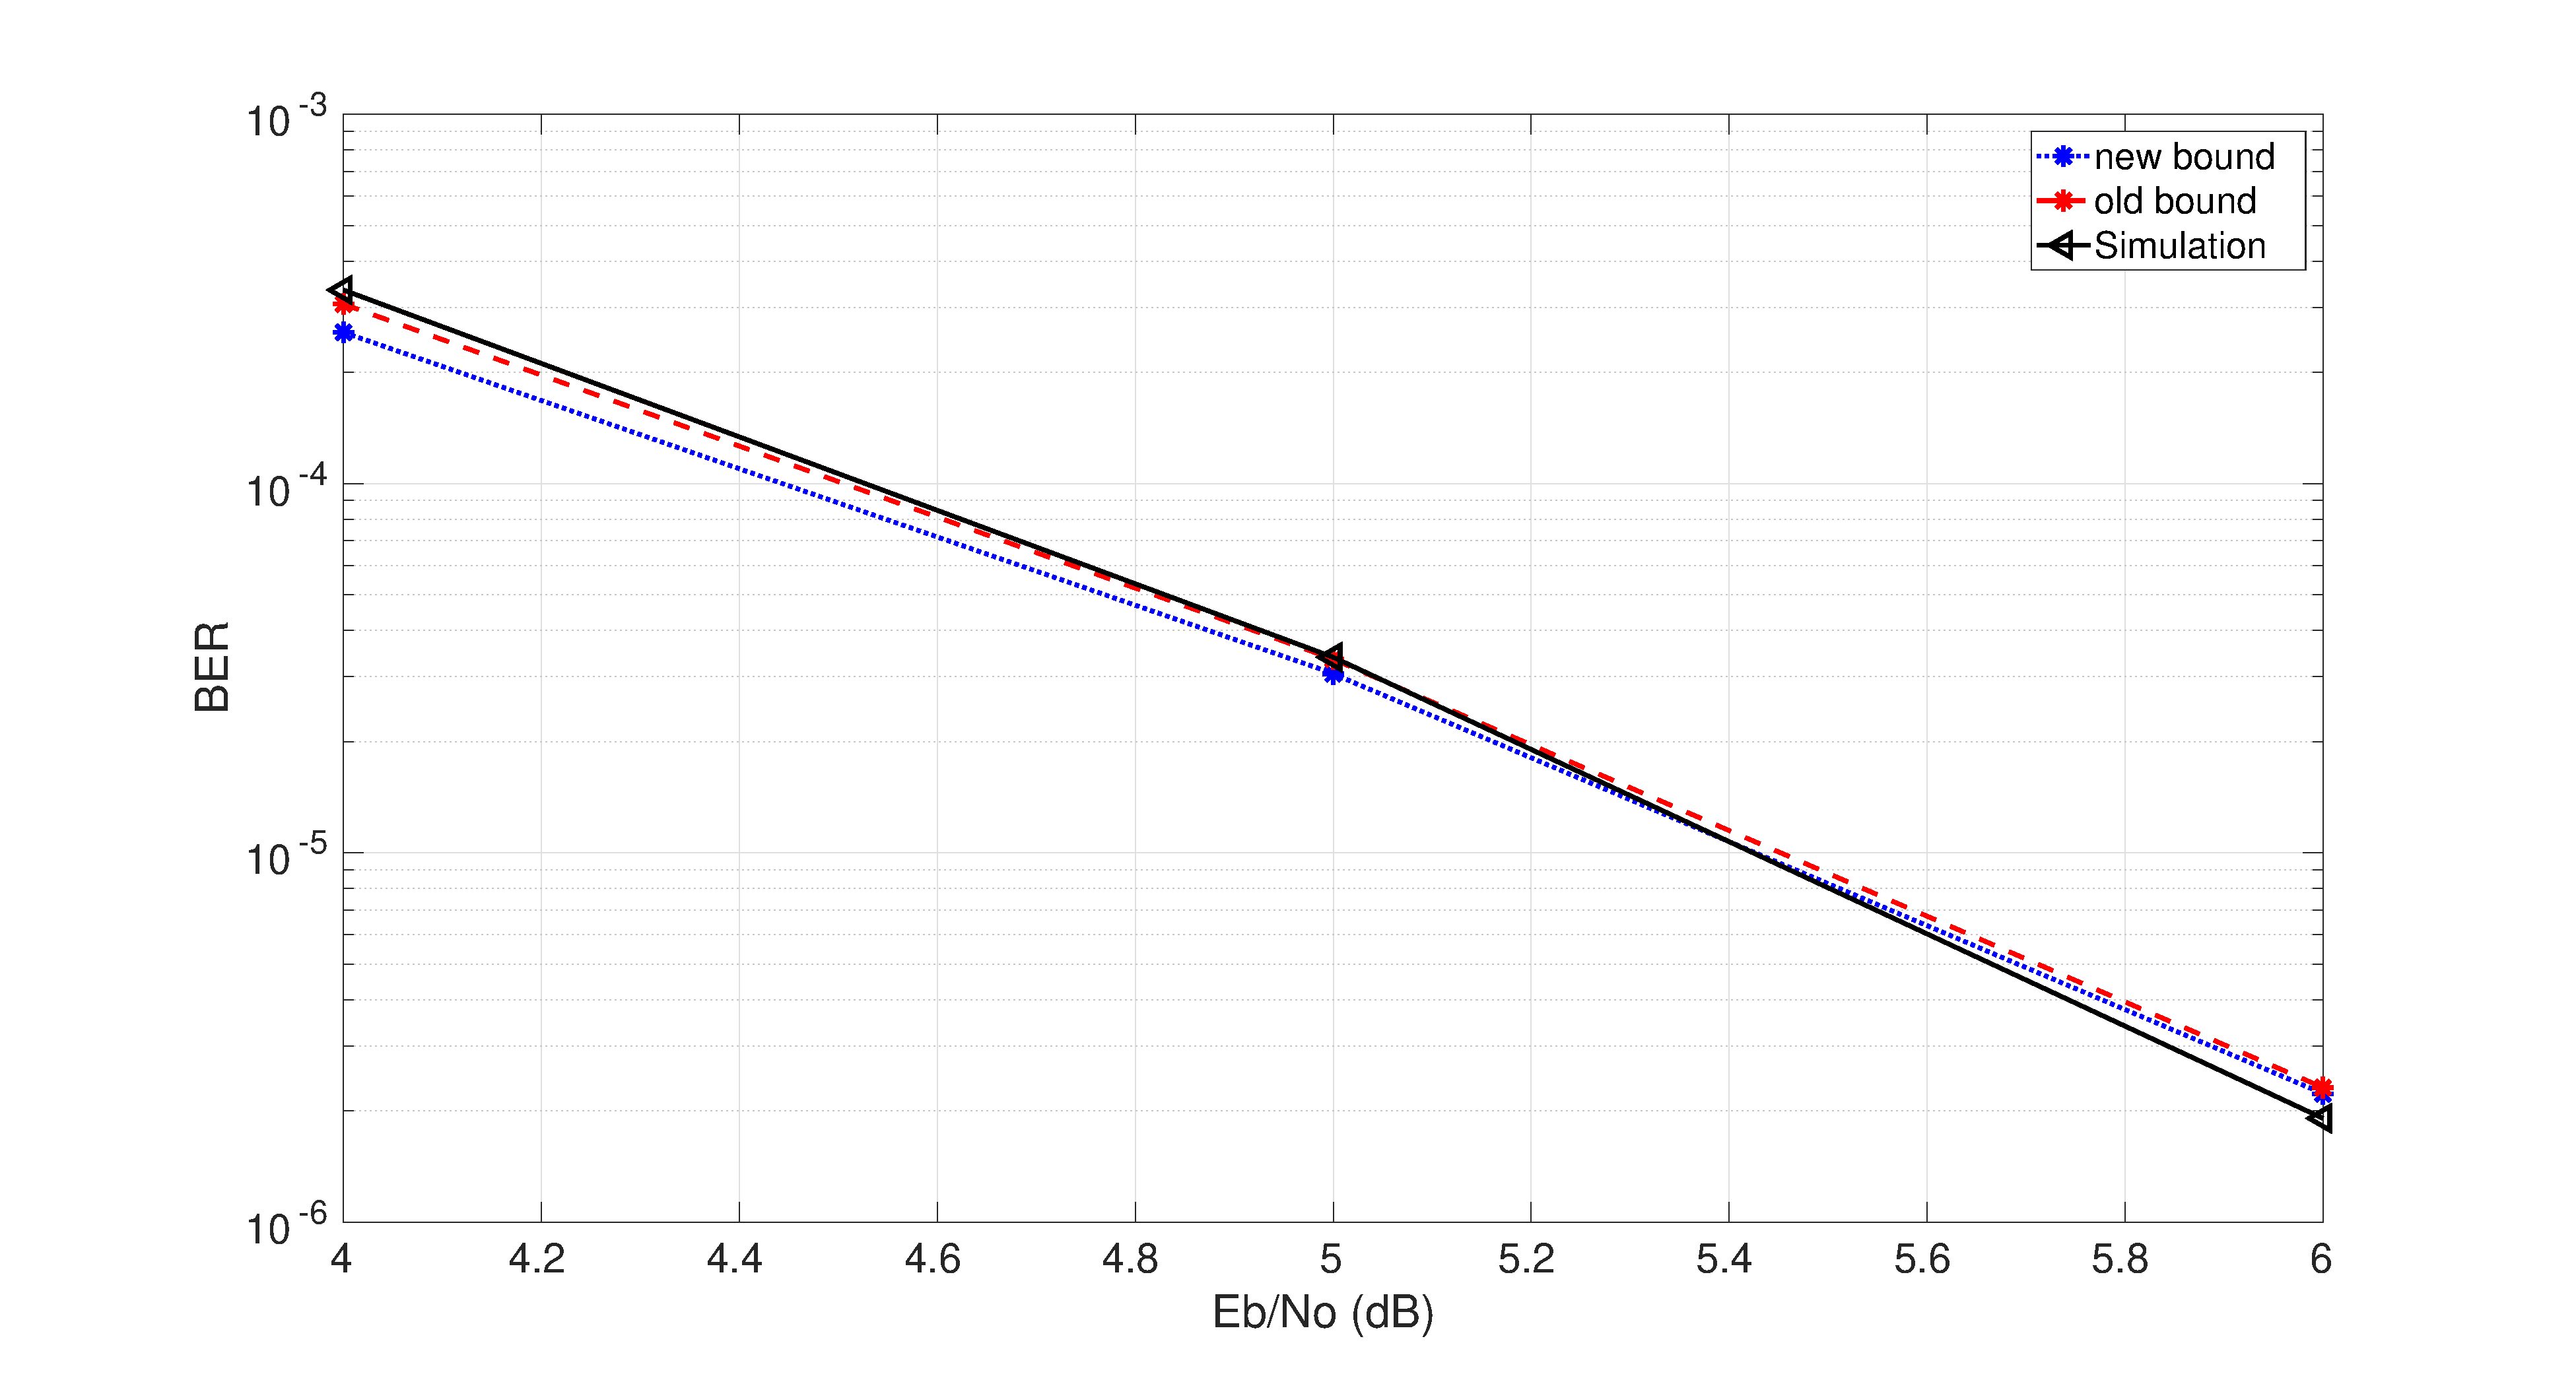
\includegraphics[width=0.5\textwidth]{./Images/RSC_37_21_v2.eps}
%\caption{Old Bound vs New Bound vs Simulation for 37/21 RSC Code, with higher weights}
%\label{simFig5}
%\end{figure}



\section{Conclusion}
\label{sec6}
In this paper, we proposed a method to determine the patterns of low-weight codewords of an RSC code. We established the low-weight codewords by identifying codewords with SCs or PCs of weight-$2$ and weight-$3$. Finally, we validated our proposed method by obtaining a union bound using the established low-weight codewords and compared it with that obtained via the transfer function method and the BER curve drawn from simulation results.

\bibliography{\folder/reference/IEEEabrv,\folder/reference/References}
\end{document}